% Numerical section for StVoWu_231004.tex.
% Include this fragment with % Numerical section for StVoWu_231004.tex.
% Include this fragment with % Numerical section for StVoWu_231004.tex.
% Include this fragment with % Numerical section for StVoWu_231004.tex.
% Include this fragment with \input{numerical_section_stvowu.tex} after the
% analytical sections. It uses the article's amsart preamble and equation labels.
\section{Numerical experiments}
\label{section:numerical}

\subsection{Model, discretization, and numerical implementation}
We consider the parabolic Allen--Cahn system \eqref{allenCahn}--\eqref{allenCahnboundary}, with the initial conditions in \eqref{initialConditions}. In the computations, the bulk and surface nonlinearities are chosen as
\begin{equation}
\label{num:potential}
\begin{aligned}
 f(u)&=u^3-u=F'(u), & F(u)&=\frac14(u^2-1)^2,\\
 g(u^\Gamma)&=\beta\bigl((u^\Gamma)^3-u^\Gamma\bigr)=G'(u^\Gamma), &
 G(u^\Gamma)&=\frac{\beta}{4}\bigl((u^\Gamma)^2-1\bigr)^2.
\end{aligned}
\end{equation}
where $\beta>0$ weights the surface potential. The corresponding total energy is
\begin{equation}
\label{num:energy}
\mathcal E(u,u^\Gamma)=\int_\Omega\left(\frac12|\nabla u|^2+F(u)\right)\,\d x
+\int_\Gamma\left(\frac12|\nabla_\Gamma u^\Gamma|^2+G(u^\Gamma)\right)\,\d\sigma.
\end{equation}
All variables and parameters below are dimensionless.

Although the paper treats domains in $\mathbb R^3$, the computations reported here use a two-dimensional rectangular domain $\Omega=(0,2)\times(0,1)$ and its full boundary $\Gamma=\partial\Omega$. The bulk is discretized by bilinear quadrilateral $Q_1$ elements, with the same scalar degrees of freedom used by the boundary line elements. Nine Gauss points are used in each quadrilateral to integrate the cubic reaction term, and three points are used on each line element. The direct evolution problem is solved by the C++ OOFEM transport solver with $\alpha=1$ and input tolerance $\mathrm{rtol}=10^{-11}$. The WED trajectories are computed by a separate Python minimizer; they are not computed by the OOFEM executable. The minimizer uses piecewise-linear time elements, Gaussian quadrature, a free terminal value, and damped sparse Newton iterations. Its stopping tolerance is the infinity norm of the gradient of the rescaled functional, and the maximum number of iterations is 100.

Following the time rescaling used in the proof of the WED result, let $s=t/\eps$. The finite-horizon functional minimized in the computations is
\begin{equation}
\label{num:wed}
\begin{split}
J_{\eps,S_{\max}}(v)=\int_0^{S_{\max}}e^{-s}\bigg[&\frac12\|v_s\|^2_{L^2(\Omega)\oplus L^2(\Gamma)}\\
&+\frac{\eps}{2}\|\nabla v\|^2_{L^2(\Omega)}
+\frac{\eps}{2}\|\nabla_\Gamma v^\Gamma\|^2_{L^2(\Gamma)}\\
&+\eps\int_\Omega F(v)\,\d x
+\eps\int_\Gamma G(v^\Gamma)\,\d\sigma\bigg],\d s,
\end{split}
\end{equation}
subject to $v(0)=u^0$ and $v^\Gamma=v|_\Gamma$. The terminal value at $s=S_{\max}$ is unconstrained. This is a truncated and discretized counterpart of the WED formulation underlying Theorem~\ref{WEDapproach}; the corresponding Euler--Lagrange equation is discussed in \eqref{55b}. The step in physical time satisfies
\begin{equation}
\label{num:dt}
\Delta t=\eps\,\Delta s.
\end{equation}

The nonuniform initial profile used for the WED limit, horizon, spatial, and $\beta$ studies is
\begin{equation}
\label{num:initial}
u^0(x,y)=0.2+0.1\left[\cos\!\left(\frac{\pi x}{2}\right)\cos(\pi y)
+0.25\sin\!\left(\frac{\pi x}{2}\right)\sin(\pi y)\right],
\end{equation}
with $\beta=1$ unless varied explicitly. The manufactured source is switched off for these evolution tests. In the WED limit study, the direct OOFEM trajectory is a numerical comparator, not an exact solution. The MMS test below is the separate comparison with a known exact solution.

\subsection{Verification of the direct solver by a manufactured solution}
We first verify the direct OOFEM solver against the manufactured solution
\begin{equation}
\label{num:mms}
u^*(x,y,t)=0.2+0.1e^{-t}\left[\cos\!\left(\frac{\pi x}{2}\right)\cos(\pi y)
+0.25\sin\!\left(\frac{\pi x}{2}\right)\sin(\pi y)\right],
\end{equation}
with consistent source terms in the bulk and on the boundary. Here $\eps$ is not a parameter of the direct evolution; the time step is $\Delta t=5\,10^{-4}$, the final time is $T=0.02$, and $\beta=1$. The reported nodal RMS error is $e_h=[N^{-1}\sum_{i=1}^N|u_i-u^*(x_i,T)|^2]^{1/2}$. The observed slope $p=\log_2(e_h/e_{h/2})$ is empirical.
\begin{center}\small
\begin{tabular}{rrrrrrr}
\hline
Mesh & Nodes/DoFs & $h$ & Nodal RMS & Maximum error & $\Delta t$ & $p$\\
\hline
$8\times4$ &45&0.250&$7.8821\,10^{-5}$&$1.8014\,10^{-4}$&$5\,10^{-4}$&--\\
$16\times8$&153&0.125&$1.7886\,10^{-5}$&$3.8000\,10^{-5}$&$5\,10^{-4}$&2.140\\
$32\times16$&561&0.0625&$4.3869\,10^{-6}$&$9.4361\,10^{-6}$&$5\,10^{-4}$&2.028\\
\hline
\end{tabular}
\end{center}
The observed order is consistent with second-order spatial convergence for the direct solver in this MMS case. This test verifies the direct solver and does not validate the WED minimizer.

\subsection{Dissipation and the discrete energy balance}
For the unforced gradient-flow system, the formal energy identity associated with \eqref{allenCahn}--\eqref{allenCahnboundary} is
\begin{equation}
\label{num:formal-dissipation}
\frac{\d}{\d t}\mathcal E(u(t),u^\Gamma(t))
=-\|u_t(t)\|_{L^2(\Omega)}^2-\|u_t^\Gamma(t)\|_{L^2(\Gamma)}^2.
\end{equation}
We define the accumulated bulk and boundary dissipations and the balance residual by
\begin{equation}
\label{num:balance}
D_\Omega=\int_0^T\!\int_\Omega|u_t|^2\,\d x\,\d t,\qquad
D_\Gamma=\int_0^T\!\int_\Gamma|u_t^\Gamma|^2\,\d\sigma\,\d t,\qquad
R_E=\mathcal E(T)-\mathcal E(0)+D_\Omega+D_\Gamma.
\end{equation}
The energy-balance runs use $T=0.1$, $\Omega=(0,1)^2$, a $20\times20$ quadrilateral mesh, $u^0(x,y)=0.1+0.05\cos(2\pi x)$, $\beta=1$, and no manufactured source. The values of $u_t$ are approximated by backward differences and the dissipations are evaluated using the FEM mass matrices. Thus, this is a discrete finite-step check, not an analytical proof of stability.
\begin{center}\small
\begin{tabular}{rrrrrrr}
\hline
$\Delta t$&$\mathcal E(0)$&$\mathcal E(T)$&$D_\Omega$&$D_\Gamma$&$R_E$&$|R_E|/\mathcal E(0)$\\
\hline
0.00500&1.284456&1.209120&0.022138&0.047763&$-5.4350\,10^{-3}$&0.004231\\
0.00250&1.284456&1.209018&0.022887&0.049612&$-2.9395\,10^{-3}$&0.002289\\
0.00125&1.284456&1.208967&0.023310&0.050636&$-1.5420\,10^{-3}$&0.001201\\
\hline
\end{tabular}
\end{center}
The residual is negative and its normalized absolute value decreases from $0.423\%$ to $0.120\%$ as the time step is refined. Since $u_t$ and the dissipations are numerically approximated, a nonzero residual at finite step size is expected. Figure~\ref{num:fig-energy} shows the bulk and surface contributions and their sum; no monotonicity is expected of each contribution separately.

\subsection{The limit $\eps\to0$ for WED minimizers}
We compare the WED paths with a direct OOFEM path on the same $8\times4$ mesh. Both are interpolated to the common physical-time window $t\in[0,0.1]$. The bulk and boundary errors are
\begin{equation}
\label{num:errors}
\begin{split}
E_\Omega&=\left(\int_0^{0.1}\|u_{\rm WED}(t)-u_{\rm OOFEM}(t)\|^2_{L^2(\Omega)}\,\d t\right)^{1/2},\\
E_\Gamma&=\left(\int_0^{0.1}\|u^\Gamma_{\rm WED}(t)-u^\Gamma_{\rm OOFEM}(t)\|^2_{L^2(\Gamma)}\,\d t\right)^{1/2}.
\end{split}
\end{equation}
The direct reference uses $\Delta t=10^{-3}$. In the first series, $S_{\max}=12$, $\Delta s=0.1$, tolerance $2\,10^{-5}$, and the mesh are fixed; hence $\Delta t$ varies with $\eps$ by \eqref{num:dt}. In the second series, $\Delta t=0.005$ is fixed and $\Delta s=0.005/\eps$; $S_{\max}=12$, the mesh, and tolerance remain fixed. Every run converges in two Newton iterations. The local slopes are empirical estimates, not theoretical orders.
\begin{center}\scriptsize
\begin{tabular}{llrrrrrrr}
\hline
Series&$\eps$&$\Delta s$&$\Delta t$&$\eps S_{\max}$&$E_\Omega$&$E_\Gamma$&Newton&tol\\
\hline
fixed $\Delta s$&0.1000&0.100&0.0100&1.200&$1.8485\,10^{-3}$&$3.1960\,10^{-3}$&2&$2\,10^{-5}$\\
&0.0500&0.100&0.0050&0.600&$1.1511\,10^{-3}$&$2.0198\,10^{-3}$&2&$2\,10^{-5}$\\
&0.0250&0.100&0.0025&0.300&$6.8730\,10^{-4}$&$1.1978\,10^{-3}$&2&$2\,10^{-5}$\\
&0.0125&0.100&0.00125&0.150&$3.8735\,10^{-4}$&$6.6759\,10^{-4}$&2&$2\,10^{-5}$\\
fixed $\Delta t$&0.1000&0.050&0.0050&1.200&$1.8475\,10^{-3}$&$3.1947\,10^{-3}$&2&$2\,10^{-5}$\\
&0.0500&0.100&0.0050&0.600&$1.1511\,10^{-3}$&$2.0198\,10^{-3}$&2&$2\,10^{-5}$\\
&0.0250&0.200&0.0050&0.300&$6.8614\,10^{-4}$&$1.1959\,10^{-3}$&2&$2\,10^{-5}$\\
&0.0125&0.400&0.0050&0.150&$3.8299\,10^{-4}$&$6.6022\,10^{-4}$&2&$2\,10^{-5}$\\
\hline
\end{tabular}
\end{center}
For fixed $\Delta s$, the bulk/boundary local slopes are $0.68/0.66$, $0.74/0.75$, and $0.83/0.84$. For fixed physical $\Delta t$, they are approximately $0.68/0.66$, $0.75/0.76$, and $0.84/0.86$. The decreasing error trend is similar under both protocols. Keeping $\Delta t$ fixed reduces temporal-step confounding but does not remove all temporal error; for $\eps=0.0125$ it gives the relatively coarse rescaled step $\Delta s=0.4$.

We therefore additionally halve $\Delta s$ from $0.4$ to $0.2$ at $\eps=0.0125$, keeping $S_{\max}=12$, the mesh, and tolerance $2\,10^{-5}$ fixed. Both runs take two Newton iterations. Relative to OOFEM, the bulk error changes from $3.82985\,10^{-4}$ to $3.86483\,10^{-4}$ and the boundary error from $6.60221\,10^{-4}$ to $6.66145\,10^{-4}$, i.e., by about $0.9\%$. The space--time differences between the two WED paths are $4.16\,10^{-6}$ in the bulk and $6.44\,10^{-6}$ on the boundary. The trend is stable to this targeted refinement, while the error against OOFEM does not decrease monotonically under refinement of the time step alone; we do not interpret the slopes as asymptotic orders.
\begin{center}\small
\begin{tabular}{rrrrrr}
\hline
$\Delta s$&$\Delta t$&Newton&$E_\Omega$&$E_\Gamma$&path difference, bulk/boundary\\
\hline
0.4&0.0050&2&$3.82985\,10^{-4}$&$6.60221\,10^{-4}$&reference\\
0.2&0.0025&2&$3.86483\,10^{-4}$&$6.66145\,10^{-4}$&$4.16\,10^{-6}/6.44\,10^{-6}$\\
\hline
\end{tabular}
\end{center}
\begin{figure}[ht]\centering
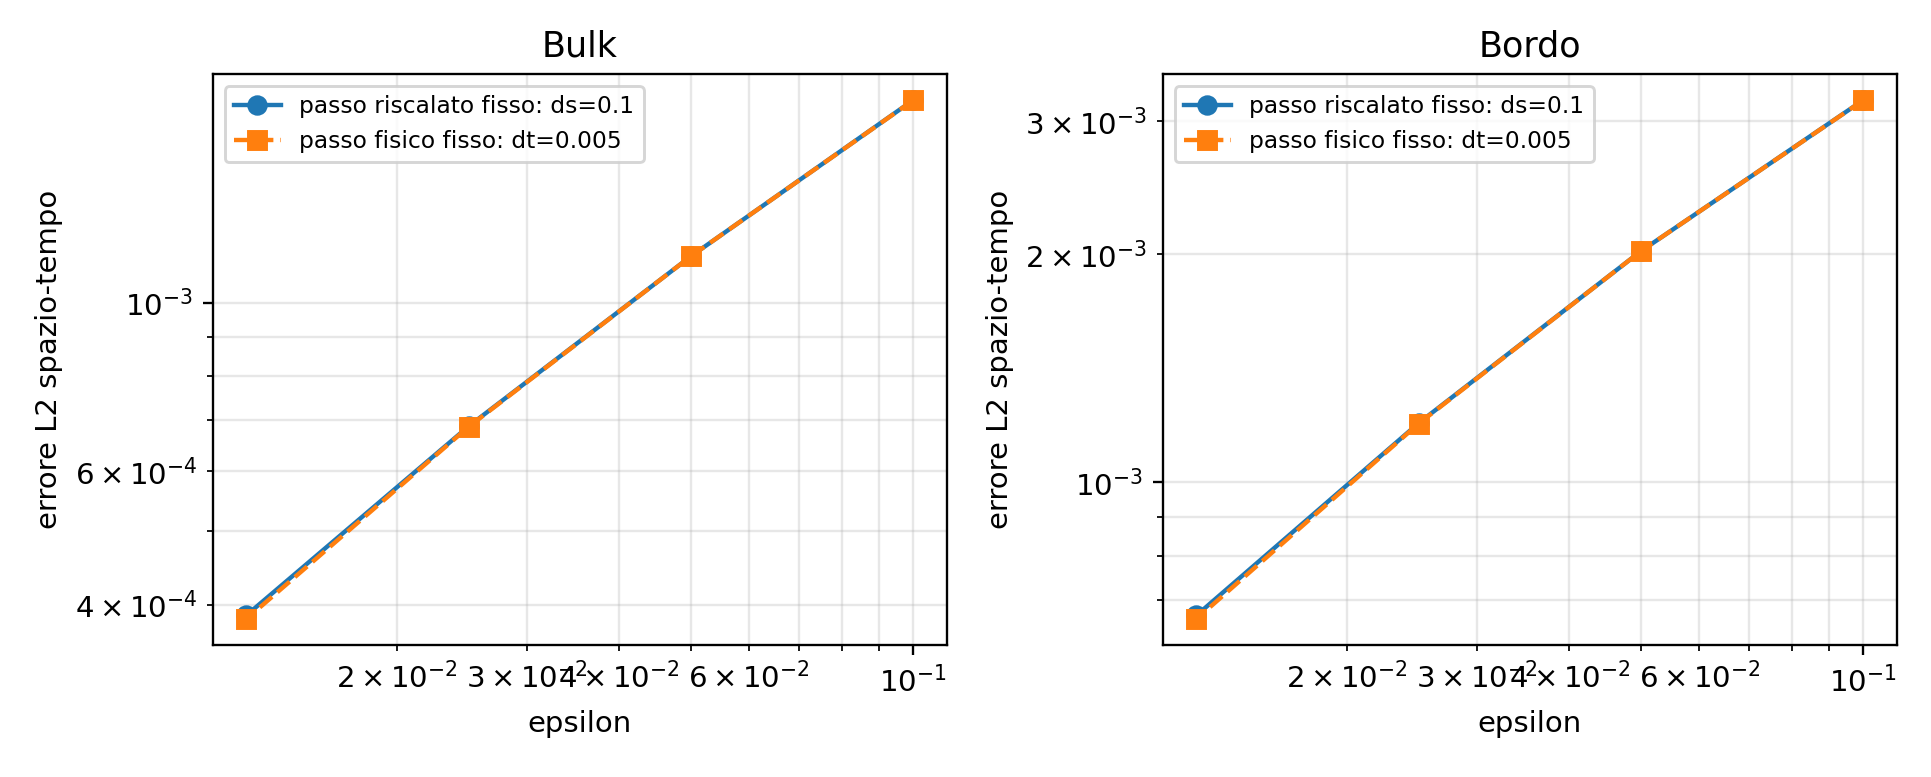
\includegraphics[width=\textwidth]{../stvowu_validation/paper_figures/figure2_epsilon.png}
\caption{Bulk and boundary errors versus $\eps$. Solid lines: fixed $\Delta s=0.1$; dashed lines: fixed physical $\Delta t=0.005$. Errors are integrated over $[0,0.1]$ relative to the direct OOFEM path with $\Delta t=0.001$.}
\label{num:fig-epsilon}\end{figure}

\subsection{Sensitivity to the finite WED horizon}
For $\eps=0.05$, $\Delta s=0.1$, tolerance $2\,10^{-5}$, and the $8\times4$ mesh, we compare $S_{\max}=6,12$ with $18$ over $t\in[0,0.1]$. The reported RMS is the nodal root-mean-square over time,
\[
\mathrm{RMS}_{S_{\max}}=\left[\int_0^{0.1}\frac1N\sum_{i=1}^N|u_i^{S_{\max}}(t)-u_i^{18}(t)|^2\,\d t\right]^{1/2},
\]
and the maximum is the largest nodal difference on the same interval.
\begin{center}\small
\begin{tabular}{rrrr}
\hline
$S_{\max}$&$\Delta t=\eps\Delta s$&RMS vs $S_{\max}=18$&maximum nodal difference\\
\hline
6&0.005&$3.6689\,10^{-5}$&$3.0215\,10^{-4}$\\
12&0.005&$1.5575\,10^{-7}$&$1.1327\,10^{-6}$\\
18&0.005&0 (reference)&0 (reference)\\
\hline
\end{tabular}
\end{center}
This is a truncation-sensitivity check for the stated initial data and time window, not a uniform estimate for other problems.
\begin{figure}[ht]\centering
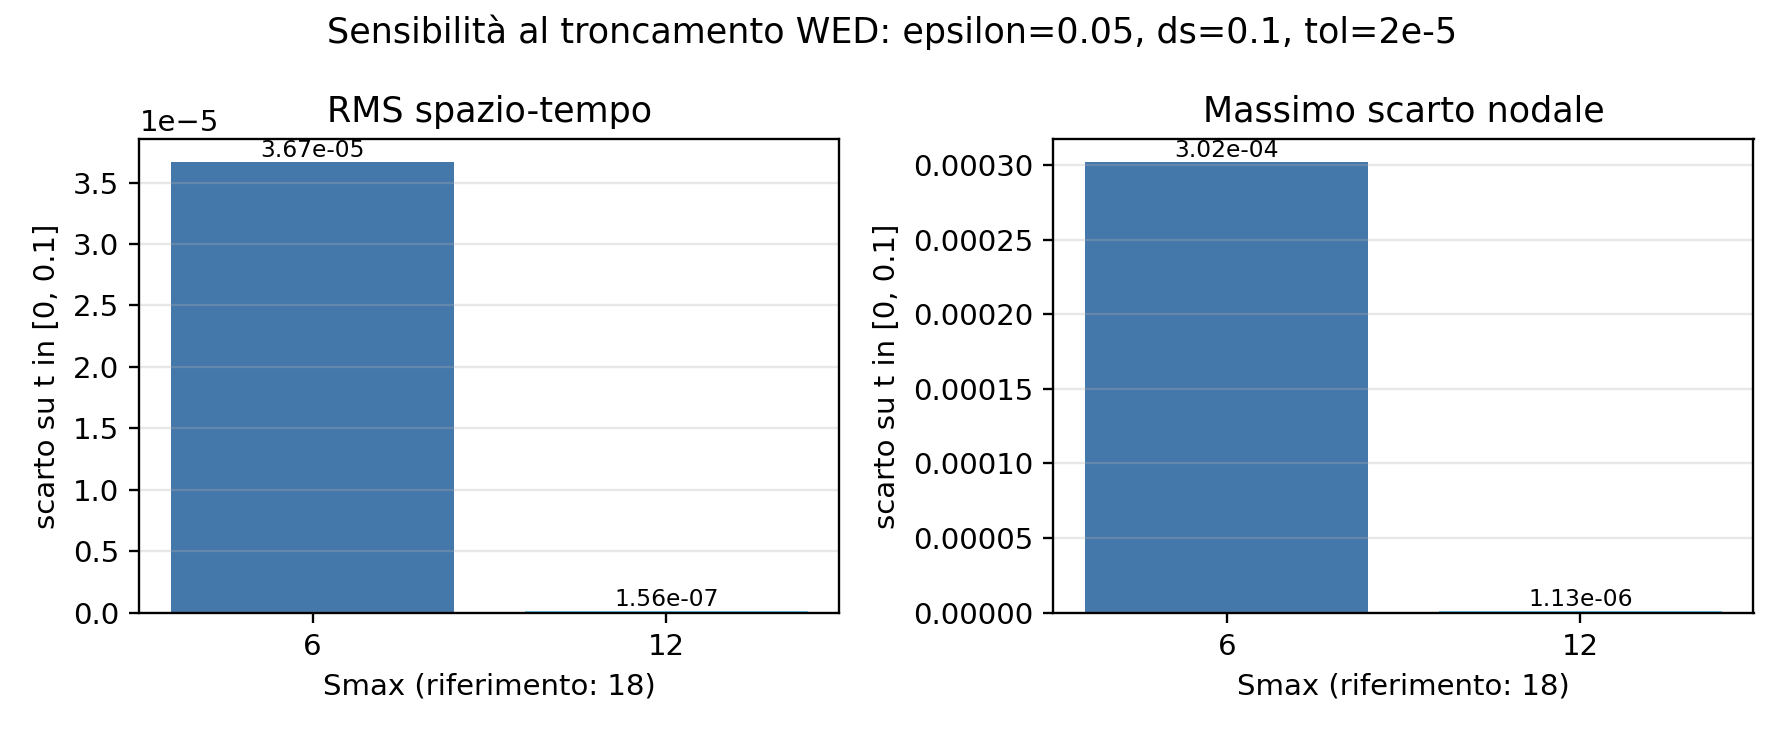
\includegraphics[width=.78\textwidth]{../stvowu_validation/paper_figures/figure3_horizon.png}
\caption{RMS and maximum nodal differences relative to $S_{\max}=18$ for $\eps=0.05$, $\Delta s=0.1$, and $t\in[0,0.1]$.}
\label{num:fig-horizon}\end{figure}

\subsection{Spatial convergence of WED paths}
At fixed $\eps=0.05$, coarse-mesh WED paths are compared against the WED path on the $32\times16$ mesh, used as a numerical reference, not an exact solution. The norms in \eqref{num:errors} are evaluated over $t\in[0,0.1]$. The baseline uses $\Delta s=0.1$ and tolerance $2\,10^{-5}$; the robustness check uses $\Delta s=0.05$ and tolerance $2\,10^{-6}$. The empirical orders are estimated from the two coarse meshes.
\begin{center}\scriptsize
\begin{tabular}{llrrrrr}
\hline
Run&Mesh&$h$&$E_\Omega$&$E_\Gamma$&$p_\Omega$&$p_\Gamma$\\
\hline
baseline&$8\times4$&0.250&$2.1961\,10^{-4}$&$3.1175\,10^{-4}$&2.107&2.243\\
&$16\times8$&0.125&$5.0963\,10^{-5}$&$6.5835\,10^{-5}$&--&--\\
&$32\times16$&0.0625&0 (reference)&0 (reference)&--&--\\
refined&$8\times4$&0.250&$2.1977\,10^{-4}$&$3.0581\,10^{-4}$&2.108&2.216\\
&$16\times8$&0.125&$5.0972\,10^{-5}$&$6.5840\,10^{-5}$&--&--\\
&$32\times16$&0.0625&0 (reference)&0 (reference)&--&--\\
\hline
\end{tabular}
\end{center}
The observed bulk order changes by approximately $0.001$ and the boundary order by $0.028$ under the time-step and tolerance refinement. For these meshes the trend is consistent with second-order spatial convergence and is stable under the tested refinement. WED/OOFEM differences include the finite-$\eps$ bias and are not used to infer spatial order.
\begin{figure}[ht]\centering
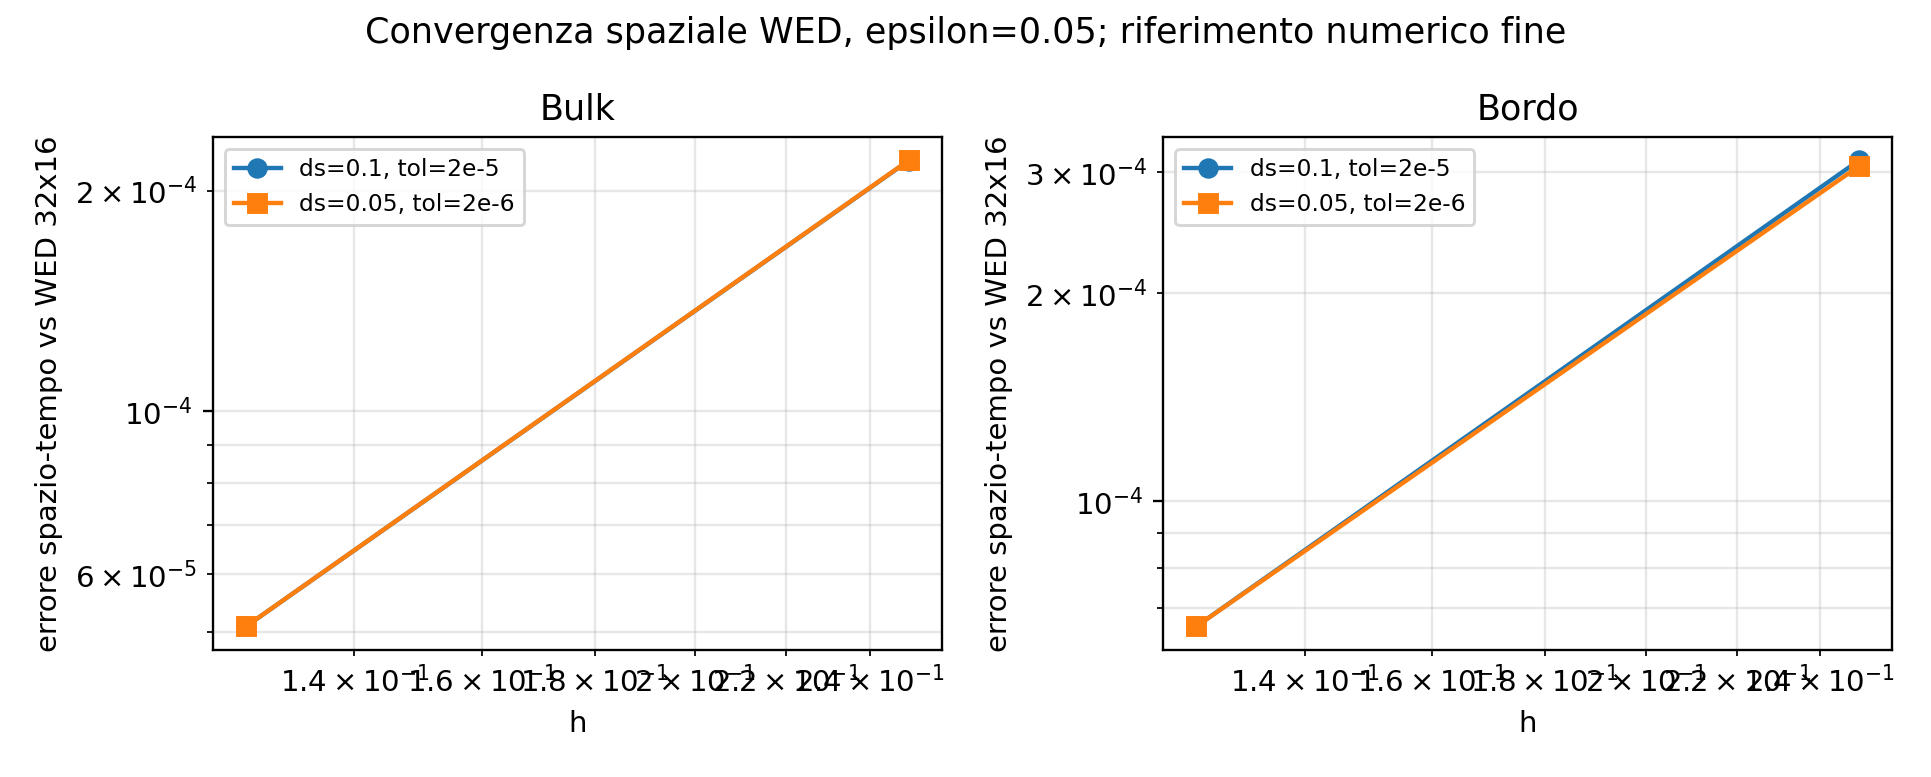
\includegraphics[width=\textwidth]{../stvowu_validation/paper_figures/figure4_mesh.png}
\caption{Bulk and surface errors relative to the $32\times16$ WED path at fixed $\eps$. The fine path is a numerical reference. The two data sets use the $\Delta s$ and tolerances specified in the legend.}
\label{num:fig-mesh}\end{figure}

\subsection{Energy decay}
Figure~\ref{num:fig-energy} reports the direct evolution on $(0,1)^2$, with a $20\times20$ quadrilateral mesh, $u^0(x,y)=0.1+0.05\cos(2\pi x)$, $\beta=1$, $T=0.1$, and $\Delta t=0.00125$. The total energy decreases; no monotonicity is required of its separate bulk and boundary contributions.
\begin{figure}[ht]\centering
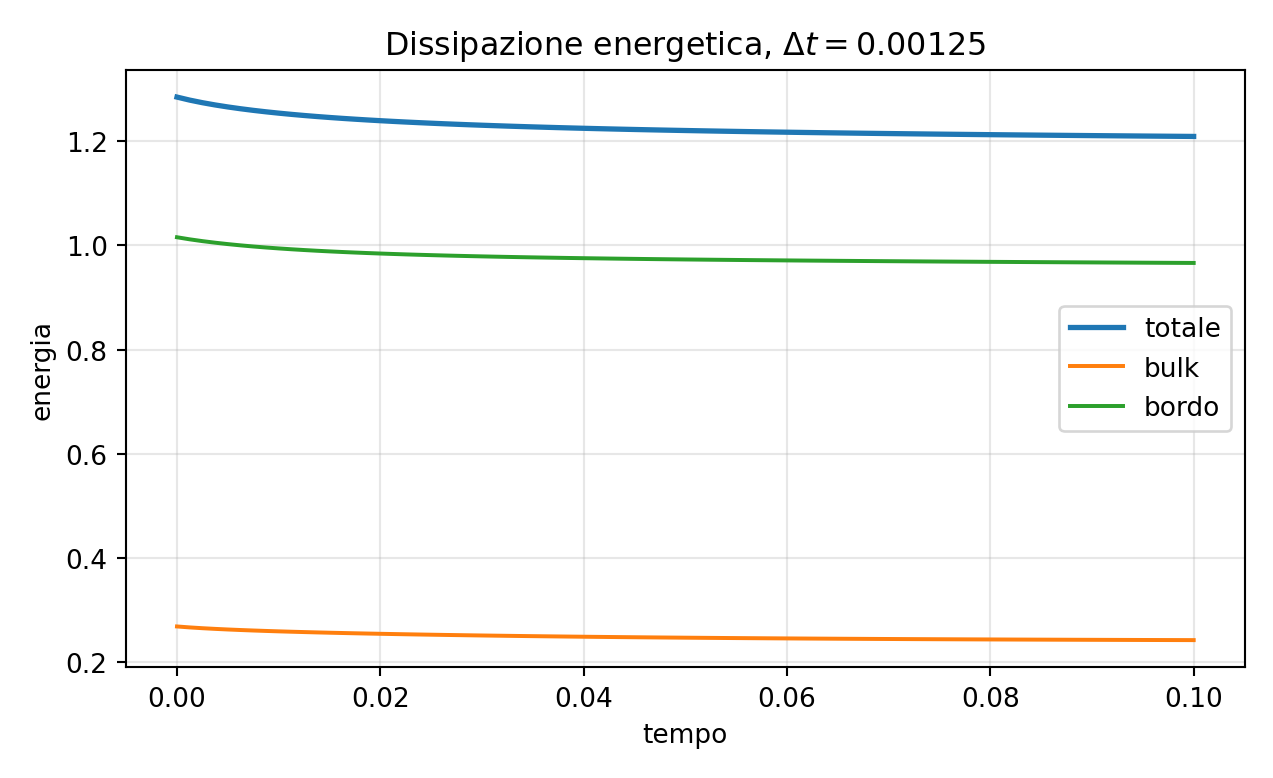
\includegraphics[width=.78\textwidth]{../stvowu_validation/paper_figures/figure5_energy.png}
\caption{Bulk, boundary, and total energy for the direct Allen--Cahn evolution on $(0,1)^2$, mesh $20\times20$, $T=0.1$, and $\Delta t=0.00125$. The total energy decreases, while the individual components need not be monotone.}
\label{num:fig-energy}\end{figure}

\subsection{Dependence on the surface parameter $\beta$}
We vary $\beta\in\{0.5,1,2,5\}$ while keeping the domain $(0,2)\times(0,1)$, mesh $8\times4$, initial profile \eqref{num:initial}, and disabled manufactured source fixed. The direct OOFEM runs use $\Delta t=5\,10^{-4}$ and end at $T=0.02$. The WED runs use $\eps=0.05$, $S_{\max}=4$, $\Delta s=0.1$, tolerance $2\,10^{-5}$, and end at physical time $T=0.2$. Since the final times differ, the two series are presented separately and are not compared pointwise. We denote by $M_\Gamma(T)=|\Gamma|^{-1}\int_\Gamma u^\Gamma(T)\,\d\sigma$ the boundary mean.
\begin{center}\small
\begin{tabular}{rrrrrr}
\hline
Backend, $T$&$\beta$&$M_\Gamma(T)$&$\mathcal E_\Gamma(T)$&$D_\Omega$&$D_\Gamma$\\
\hline
OOFEM, 0.02&0.5&0.202747&0.739877&0.005098&0.018408\\
&1&0.204470&1.423137&0.005238&0.020230\\
&2&0.207956&2.783037&0.006023&0.029831\\
&5&0.218748&6.806088&0.012690&0.109610\\
WED, 0.2&0.5&0.220390&--&--&--\\
&1&0.233905&--&--&--\\
&2&0.264304&--&--&--\\
&5&0.382729&--&--&--\\
\hline
\end{tabular}
\end{center}
The surface energies and dissipations are reported for the direct transient only. The results show sensitivity to $\beta$ for the selected initial condition; no universal monotonicity or relaxation time is asserted.
\begin{figure}[ht]\centering
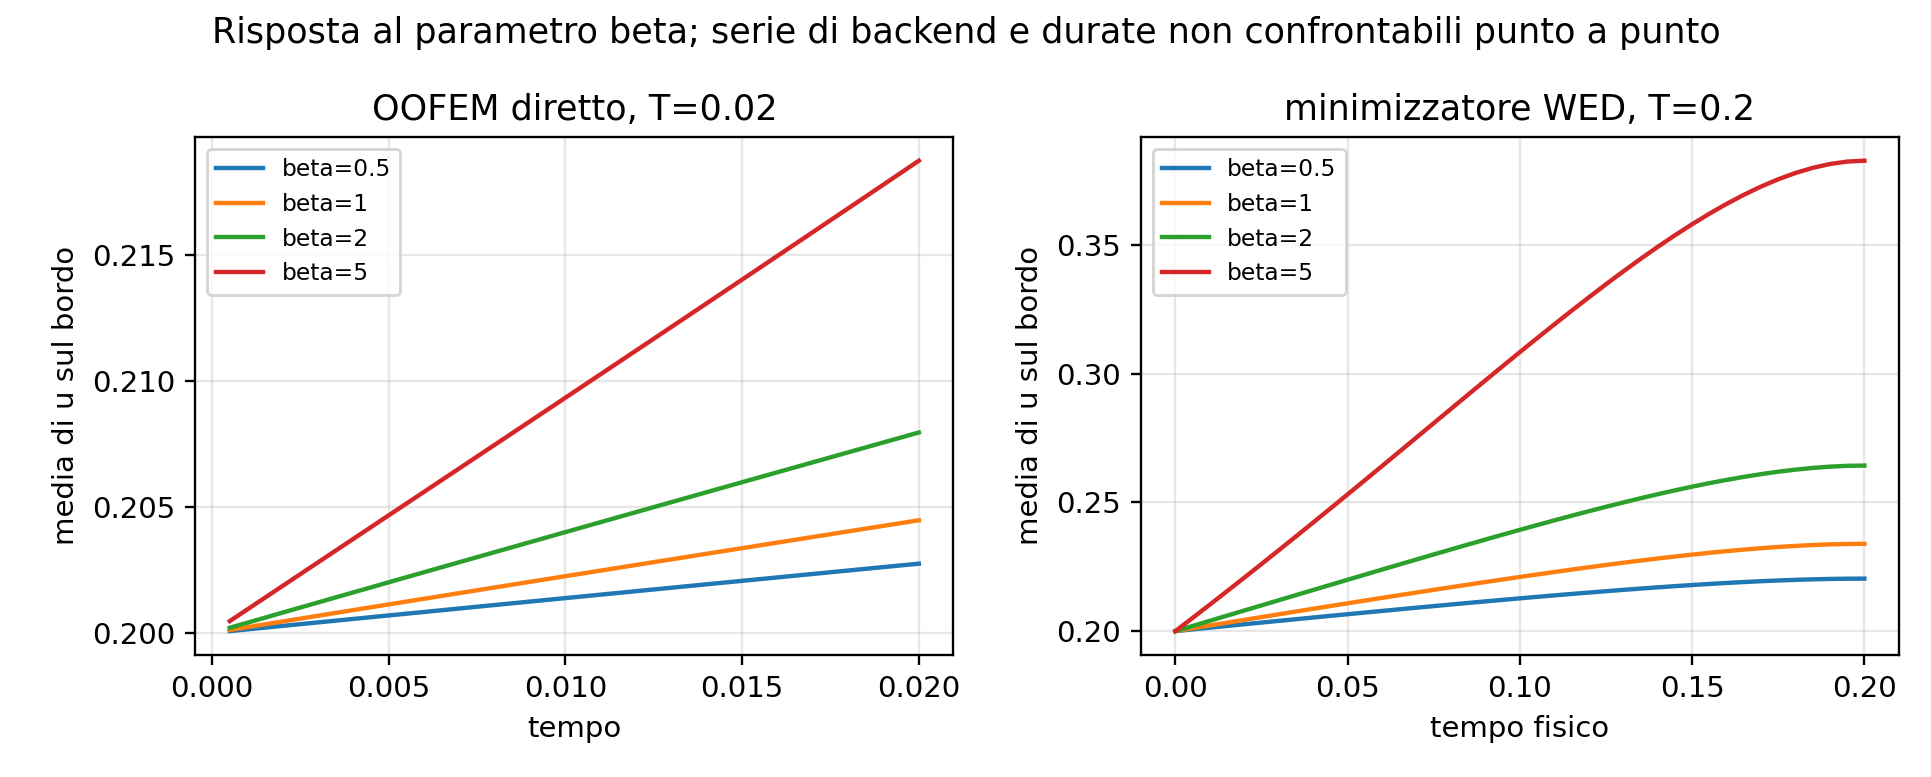
\includegraphics[width=\textwidth]{../stvowu_validation/paper_figures/figure6_beta.png}
\caption{Boundary mean for $\beta=0.5,1,2,5$. Left: direct OOFEM through $T=0.02$, $\Delta t=5\,10^{-4}$. Right: WED minimizer through $T=0.2$, $\eps=0.05$, $S_{\max}=4$, $\Delta s=0.1$. The backends and final times differ.}
\label{num:fig-beta}\end{figure}

\subsection{Scope and reproducibility}
The MMS and energy-balance checks concern the direct solver; the $\eps$, horizon, and mesh studies concern the separate WED Python minimizer. In particular, the MMS test does not validate WED. The comparison with OOFEM at finite $\eps$ includes a regularization bias and is not a pure mesh-convergence test. The reported orders are empirical estimates for the stated benchmarks and do not provide universal convergence results. The computations concern the two-dimensional parabolic model only; the semilinear-wave problem \eqref{allenCahn1} and a triangular $P_1$ benchmark are not included.

Inputs, logs, CSV data, scripts, and figures are archived in the accompanying validation directory. This section source and the six plots are stored there together with the result drivers and parameter tables. The energy residual uses backward differences on saved fields and should be interpreted as a discrete diagnostic. All conclusions are restricted to the reported geometries, initial data, meshes, and tolerances.
 after the
% analytical sections. It uses the article's amsart preamble and equation labels.
\section{Numerical experiments}
\label{section:numerical}

\subsection{Model, discretization, and numerical implementation}
We consider the parabolic Allen--Cahn system \eqref{allenCahn}--\eqref{allenCahnboundary}, with the initial conditions in \eqref{initialConditions}. In the computations, the bulk and surface nonlinearities are chosen as
\begin{equation}
\label{num:potential}
\begin{aligned}
 f(u)&=u^3-u=F'(u), & F(u)&=\frac14(u^2-1)^2,\\
 g(u^\Gamma)&=\beta\bigl((u^\Gamma)^3-u^\Gamma\bigr)=G'(u^\Gamma), &
 G(u^\Gamma)&=\frac{\beta}{4}\bigl((u^\Gamma)^2-1\bigr)^2.
\end{aligned}
\end{equation}
where $\beta>0$ weights the surface potential. The corresponding total energy is
\begin{equation}
\label{num:energy}
\mathcal E(u,u^\Gamma)=\int_\Omega\left(\frac12|\nabla u|^2+F(u)\right)\,\d x
+\int_\Gamma\left(\frac12|\nabla_\Gamma u^\Gamma|^2+G(u^\Gamma)\right)\,\d\sigma.
\end{equation}
All variables and parameters below are dimensionless.

Although the paper treats domains in $\mathbb R^3$, the computations reported here use a two-dimensional rectangular domain $\Omega=(0,2)\times(0,1)$ and its full boundary $\Gamma=\partial\Omega$. The bulk is discretized by bilinear quadrilateral $Q_1$ elements, with the same scalar degrees of freedom used by the boundary line elements. Nine Gauss points are used in each quadrilateral to integrate the cubic reaction term, and three points are used on each line element. The direct evolution problem is solved by the C++ OOFEM transport solver with $\alpha=1$ and input tolerance $\mathrm{rtol}=10^{-11}$. The WED trajectories are computed by a separate Python minimizer; they are not computed by the OOFEM executable. The minimizer uses piecewise-linear time elements, Gaussian quadrature, a free terminal value, and damped sparse Newton iterations. Its stopping tolerance is the infinity norm of the gradient of the rescaled functional, and the maximum number of iterations is 100.

Following the time rescaling used in the proof of the WED result, let $s=t/\eps$. The finite-horizon functional minimized in the computations is
\begin{equation}
\label{num:wed}
\begin{split}
J_{\eps,S_{\max}}(v)=\int_0^{S_{\max}}e^{-s}\bigg[&\frac12\|v_s\|^2_{L^2(\Omega)\oplus L^2(\Gamma)}\\
&+\frac{\eps}{2}\|\nabla v\|^2_{L^2(\Omega)}
+\frac{\eps}{2}\|\nabla_\Gamma v^\Gamma\|^2_{L^2(\Gamma)}\\
&+\eps\int_\Omega F(v)\,\d x
+\eps\int_\Gamma G(v^\Gamma)\,\d\sigma\bigg],\d s,
\end{split}
\end{equation}
subject to $v(0)=u^0$ and $v^\Gamma=v|_\Gamma$. The terminal value at $s=S_{\max}$ is unconstrained. This is a truncated and discretized counterpart of the WED formulation underlying Theorem~\ref{WEDapproach}; the corresponding Euler--Lagrange equation is discussed in \eqref{55b}. The step in physical time satisfies
\begin{equation}
\label{num:dt}
\Delta t=\eps\,\Delta s.
\end{equation}

The nonuniform initial profile used for the WED limit, horizon, spatial, and $\beta$ studies is
\begin{equation}
\label{num:initial}
u^0(x,y)=0.2+0.1\left[\cos\!\left(\frac{\pi x}{2}\right)\cos(\pi y)
+0.25\sin\!\left(\frac{\pi x}{2}\right)\sin(\pi y)\right],
\end{equation}
with $\beta=1$ unless varied explicitly. The manufactured source is switched off for these evolution tests. In the WED limit study, the direct OOFEM trajectory is a numerical comparator, not an exact solution. The MMS test below is the separate comparison with a known exact solution.

\subsection{Verification of the direct solver by a manufactured solution}
We first verify the direct OOFEM solver against the manufactured solution
\begin{equation}
\label{num:mms}
u^*(x,y,t)=0.2+0.1e^{-t}\left[\cos\!\left(\frac{\pi x}{2}\right)\cos(\pi y)
+0.25\sin\!\left(\frac{\pi x}{2}\right)\sin(\pi y)\right],
\end{equation}
with consistent source terms in the bulk and on the boundary. Here $\eps$ is not a parameter of the direct evolution; the time step is $\Delta t=5\,10^{-4}$, the final time is $T=0.02$, and $\beta=1$. The reported nodal RMS error is $e_h=[N^{-1}\sum_{i=1}^N|u_i-u^*(x_i,T)|^2]^{1/2}$. The observed slope $p=\log_2(e_h/e_{h/2})$ is empirical.
\begin{center}\small
\begin{tabular}{rrrrrrr}
\hline
Mesh & Nodes/DoFs & $h$ & Nodal RMS & Maximum error & $\Delta t$ & $p$\\
\hline
$8\times4$ &45&0.250&$7.8821\,10^{-5}$&$1.8014\,10^{-4}$&$5\,10^{-4}$&--\\
$16\times8$&153&0.125&$1.7886\,10^{-5}$&$3.8000\,10^{-5}$&$5\,10^{-4}$&2.140\\
$32\times16$&561&0.0625&$4.3869\,10^{-6}$&$9.4361\,10^{-6}$&$5\,10^{-4}$&2.028\\
\hline
\end{tabular}
\end{center}
The observed order is consistent with second-order spatial convergence for the direct solver in this MMS case. This test verifies the direct solver and does not validate the WED minimizer.

\subsection{Dissipation and the discrete energy balance}
For the unforced gradient-flow system, the formal energy identity associated with \eqref{allenCahn}--\eqref{allenCahnboundary} is
\begin{equation}
\label{num:formal-dissipation}
\frac{\d}{\d t}\mathcal E(u(t),u^\Gamma(t))
=-\|u_t(t)\|_{L^2(\Omega)}^2-\|u_t^\Gamma(t)\|_{L^2(\Gamma)}^2.
\end{equation}
We define the accumulated bulk and boundary dissipations and the balance residual by
\begin{equation}
\label{num:balance}
D_\Omega=\int_0^T\!\int_\Omega|u_t|^2\,\d x\,\d t,\qquad
D_\Gamma=\int_0^T\!\int_\Gamma|u_t^\Gamma|^2\,\d\sigma\,\d t,\qquad
R_E=\mathcal E(T)-\mathcal E(0)+D_\Omega+D_\Gamma.
\end{equation}
The energy-balance runs use $T=0.1$, $\Omega=(0,1)^2$, a $20\times20$ quadrilateral mesh, $u^0(x,y)=0.1+0.05\cos(2\pi x)$, $\beta=1$, and no manufactured source. The values of $u_t$ are approximated by backward differences and the dissipations are evaluated using the FEM mass matrices. Thus, this is a discrete finite-step check, not an analytical proof of stability.
\begin{center}\small
\begin{tabular}{rrrrrrr}
\hline
$\Delta t$&$\mathcal E(0)$&$\mathcal E(T)$&$D_\Omega$&$D_\Gamma$&$R_E$&$|R_E|/\mathcal E(0)$\\
\hline
0.00500&1.284456&1.209120&0.022138&0.047763&$-5.4350\,10^{-3}$&0.004231\\
0.00250&1.284456&1.209018&0.022887&0.049612&$-2.9395\,10^{-3}$&0.002289\\
0.00125&1.284456&1.208967&0.023310&0.050636&$-1.5420\,10^{-3}$&0.001201\\
\hline
\end{tabular}
\end{center}
The residual is negative and its normalized absolute value decreases from $0.423\%$ to $0.120\%$ as the time step is refined. Since $u_t$ and the dissipations are numerically approximated, a nonzero residual at finite step size is expected. Figure~\ref{num:fig-energy} shows the bulk and surface contributions and their sum; no monotonicity is expected of each contribution separately.

\subsection{The limit $\eps\to0$ for WED minimizers}
We compare the WED paths with a direct OOFEM path on the same $8\times4$ mesh. Both are interpolated to the common physical-time window $t\in[0,0.1]$. The bulk and boundary errors are
\begin{equation}
\label{num:errors}
\begin{split}
E_\Omega&=\left(\int_0^{0.1}\|u_{\rm WED}(t)-u_{\rm OOFEM}(t)\|^2_{L^2(\Omega)}\,\d t\right)^{1/2},\\
E_\Gamma&=\left(\int_0^{0.1}\|u^\Gamma_{\rm WED}(t)-u^\Gamma_{\rm OOFEM}(t)\|^2_{L^2(\Gamma)}\,\d t\right)^{1/2}.
\end{split}
\end{equation}
The direct reference uses $\Delta t=10^{-3}$. In the first series, $S_{\max}=12$, $\Delta s=0.1$, tolerance $2\,10^{-5}$, and the mesh are fixed; hence $\Delta t$ varies with $\eps$ by \eqref{num:dt}. In the second series, $\Delta t=0.005$ is fixed and $\Delta s=0.005/\eps$; $S_{\max}=12$, the mesh, and tolerance remain fixed. Every run converges in two Newton iterations. The local slopes are empirical estimates, not theoretical orders.
\begin{center}\scriptsize
\begin{tabular}{llrrrrrrr}
\hline
Series&$\eps$&$\Delta s$&$\Delta t$&$\eps S_{\max}$&$E_\Omega$&$E_\Gamma$&Newton&tol\\
\hline
fixed $\Delta s$&0.1000&0.100&0.0100&1.200&$1.8485\,10^{-3}$&$3.1960\,10^{-3}$&2&$2\,10^{-5}$\\
&0.0500&0.100&0.0050&0.600&$1.1511\,10^{-3}$&$2.0198\,10^{-3}$&2&$2\,10^{-5}$\\
&0.0250&0.100&0.0025&0.300&$6.8730\,10^{-4}$&$1.1978\,10^{-3}$&2&$2\,10^{-5}$\\
&0.0125&0.100&0.00125&0.150&$3.8735\,10^{-4}$&$6.6759\,10^{-4}$&2&$2\,10^{-5}$\\
fixed $\Delta t$&0.1000&0.050&0.0050&1.200&$1.8475\,10^{-3}$&$3.1947\,10^{-3}$&2&$2\,10^{-5}$\\
&0.0500&0.100&0.0050&0.600&$1.1511\,10^{-3}$&$2.0198\,10^{-3}$&2&$2\,10^{-5}$\\
&0.0250&0.200&0.0050&0.300&$6.8614\,10^{-4}$&$1.1959\,10^{-3}$&2&$2\,10^{-5}$\\
&0.0125&0.400&0.0050&0.150&$3.8299\,10^{-4}$&$6.6022\,10^{-4}$&2&$2\,10^{-5}$\\
\hline
\end{tabular}
\end{center}
For fixed $\Delta s$, the bulk/boundary local slopes are $0.68/0.66$, $0.74/0.75$, and $0.83/0.84$. For fixed physical $\Delta t$, they are approximately $0.68/0.66$, $0.75/0.76$, and $0.84/0.86$. The decreasing error trend is similar under both protocols. Keeping $\Delta t$ fixed reduces temporal-step confounding but does not remove all temporal error; for $\eps=0.0125$ it gives the relatively coarse rescaled step $\Delta s=0.4$.

We therefore additionally halve $\Delta s$ from $0.4$ to $0.2$ at $\eps=0.0125$, keeping $S_{\max}=12$, the mesh, and tolerance $2\,10^{-5}$ fixed. Both runs take two Newton iterations. Relative to OOFEM, the bulk error changes from $3.82985\,10^{-4}$ to $3.86483\,10^{-4}$ and the boundary error from $6.60221\,10^{-4}$ to $6.66145\,10^{-4}$, i.e., by about $0.9\%$. The space--time differences between the two WED paths are $4.16\,10^{-6}$ in the bulk and $6.44\,10^{-6}$ on the boundary. The trend is stable to this targeted refinement, while the error against OOFEM does not decrease monotonically under refinement of the time step alone; we do not interpret the slopes as asymptotic orders.
\begin{center}\small
\begin{tabular}{rrrrrr}
\hline
$\Delta s$&$\Delta t$&Newton&$E_\Omega$&$E_\Gamma$&path difference, bulk/boundary\\
\hline
0.4&0.0050&2&$3.82985\,10^{-4}$&$6.60221\,10^{-4}$&reference\\
0.2&0.0025&2&$3.86483\,10^{-4}$&$6.66145\,10^{-4}$&$4.16\,10^{-6}/6.44\,10^{-6}$\\
\hline
\end{tabular}
\end{center}
\begin{figure}[ht]\centering
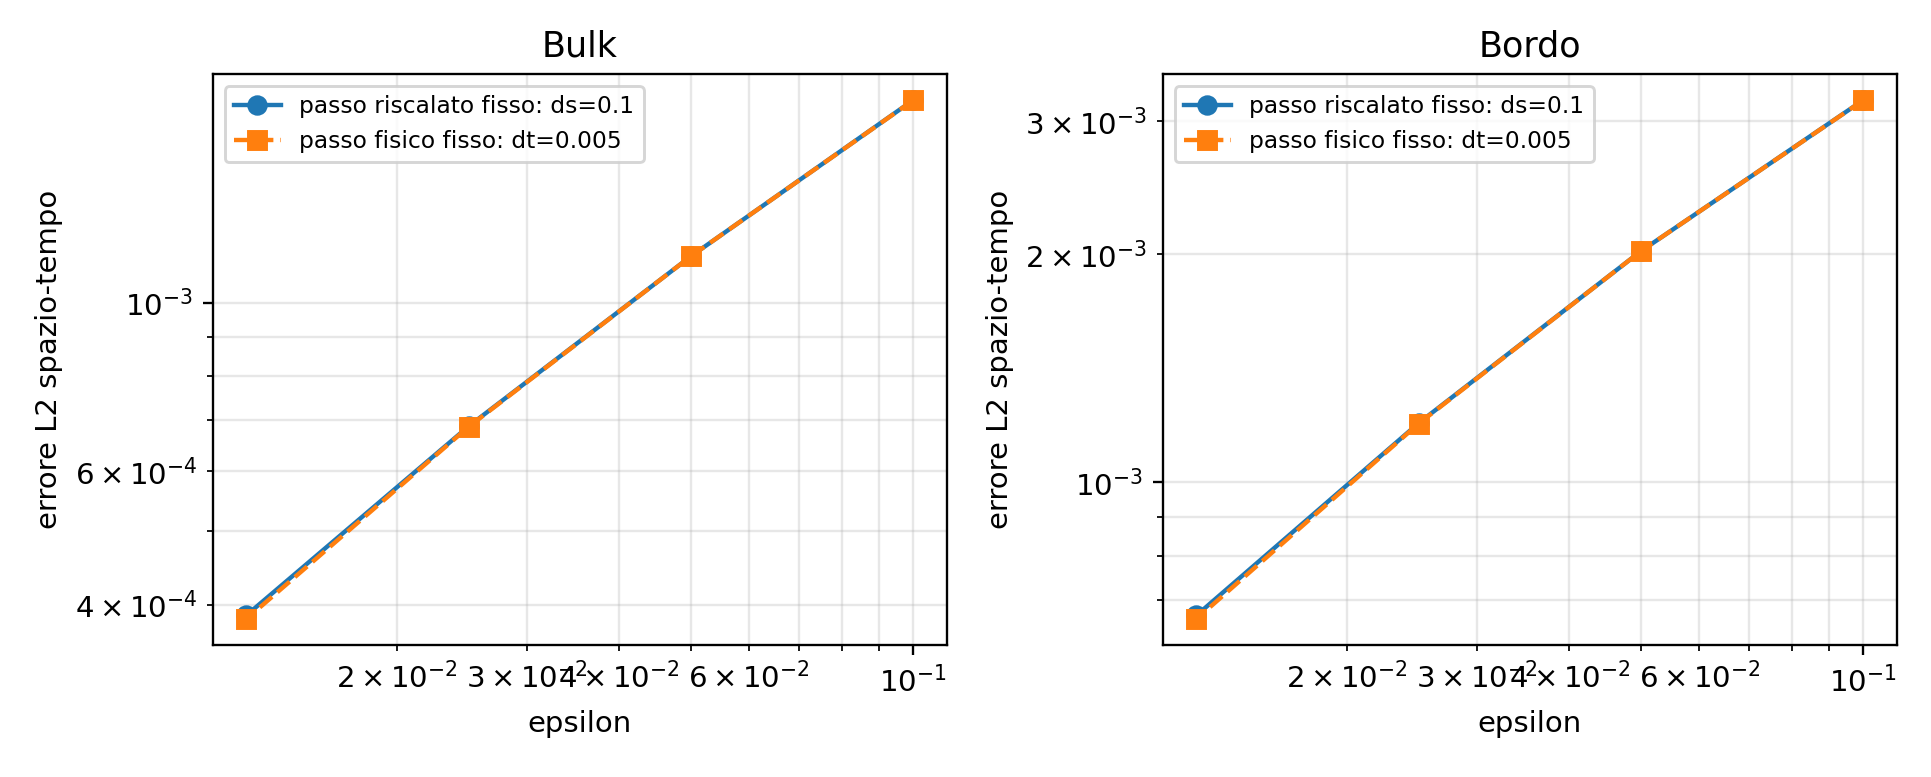
\includegraphics[width=\textwidth]{../stvowu_validation/paper_figures/figure2_epsilon.png}
\caption{Bulk and boundary errors versus $\eps$. Solid lines: fixed $\Delta s=0.1$; dashed lines: fixed physical $\Delta t=0.005$. Errors are integrated over $[0,0.1]$ relative to the direct OOFEM path with $\Delta t=0.001$.}
\label{num:fig-epsilon}\end{figure}

\subsection{Sensitivity to the finite WED horizon}
For $\eps=0.05$, $\Delta s=0.1$, tolerance $2\,10^{-5}$, and the $8\times4$ mesh, we compare $S_{\max}=6,12$ with $18$ over $t\in[0,0.1]$. The reported RMS is the nodal root-mean-square over time,
\[
\mathrm{RMS}_{S_{\max}}=\left[\int_0^{0.1}\frac1N\sum_{i=1}^N|u_i^{S_{\max}}(t)-u_i^{18}(t)|^2\,\d t\right]^{1/2},
\]
and the maximum is the largest nodal difference on the same interval.
\begin{center}\small
\begin{tabular}{rrrr}
\hline
$S_{\max}$&$\Delta t=\eps\Delta s$&RMS vs $S_{\max}=18$&maximum nodal difference\\
\hline
6&0.005&$3.6689\,10^{-5}$&$3.0215\,10^{-4}$\\
12&0.005&$1.5575\,10^{-7}$&$1.1327\,10^{-6}$\\
18&0.005&0 (reference)&0 (reference)\\
\hline
\end{tabular}
\end{center}
This is a truncation-sensitivity check for the stated initial data and time window, not a uniform estimate for other problems.
\begin{figure}[ht]\centering
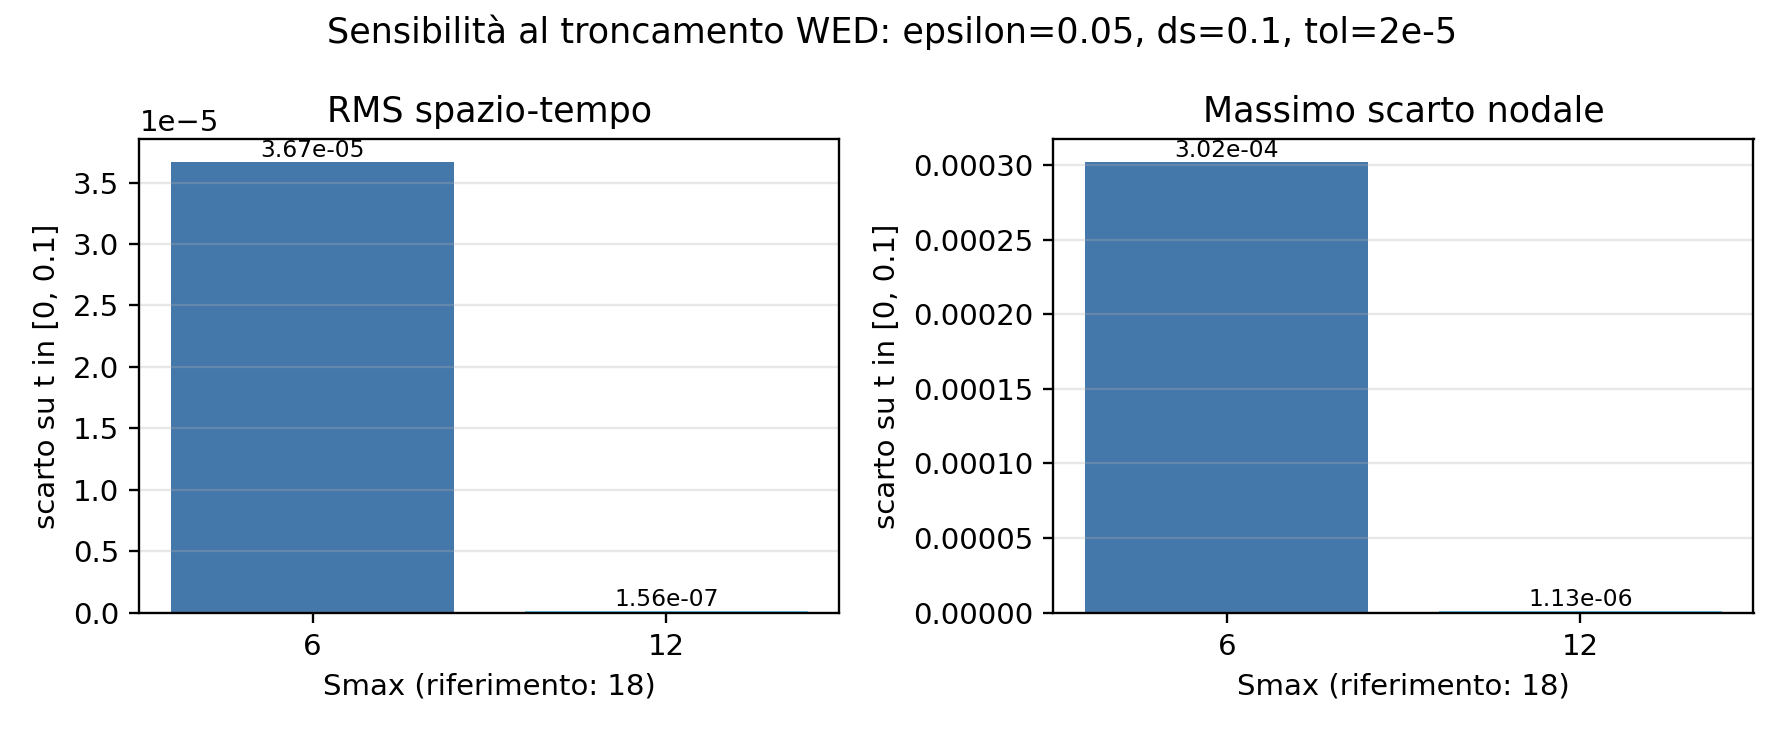
\includegraphics[width=.78\textwidth]{../stvowu_validation/paper_figures/figure3_horizon.png}
\caption{RMS and maximum nodal differences relative to $S_{\max}=18$ for $\eps=0.05$, $\Delta s=0.1$, and $t\in[0,0.1]$.}
\label{num:fig-horizon}\end{figure}

\subsection{Spatial convergence of WED paths}
At fixed $\eps=0.05$, coarse-mesh WED paths are compared against the WED path on the $32\times16$ mesh, used as a numerical reference, not an exact solution. The norms in \eqref{num:errors} are evaluated over $t\in[0,0.1]$. The baseline uses $\Delta s=0.1$ and tolerance $2\,10^{-5}$; the robustness check uses $\Delta s=0.05$ and tolerance $2\,10^{-6}$. The empirical orders are estimated from the two coarse meshes.
\begin{center}\scriptsize
\begin{tabular}{llrrrrr}
\hline
Run&Mesh&$h$&$E_\Omega$&$E_\Gamma$&$p_\Omega$&$p_\Gamma$\\
\hline
baseline&$8\times4$&0.250&$2.1961\,10^{-4}$&$3.1175\,10^{-4}$&2.107&2.243\\
&$16\times8$&0.125&$5.0963\,10^{-5}$&$6.5835\,10^{-5}$&--&--\\
&$32\times16$&0.0625&0 (reference)&0 (reference)&--&--\\
refined&$8\times4$&0.250&$2.1977\,10^{-4}$&$3.0581\,10^{-4}$&2.108&2.216\\
&$16\times8$&0.125&$5.0972\,10^{-5}$&$6.5840\,10^{-5}$&--&--\\
&$32\times16$&0.0625&0 (reference)&0 (reference)&--&--\\
\hline
\end{tabular}
\end{center}
The observed bulk order changes by approximately $0.001$ and the boundary order by $0.028$ under the time-step and tolerance refinement. For these meshes the trend is consistent with second-order spatial convergence and is stable under the tested refinement. WED/OOFEM differences include the finite-$\eps$ bias and are not used to infer spatial order.
\begin{figure}[ht]\centering
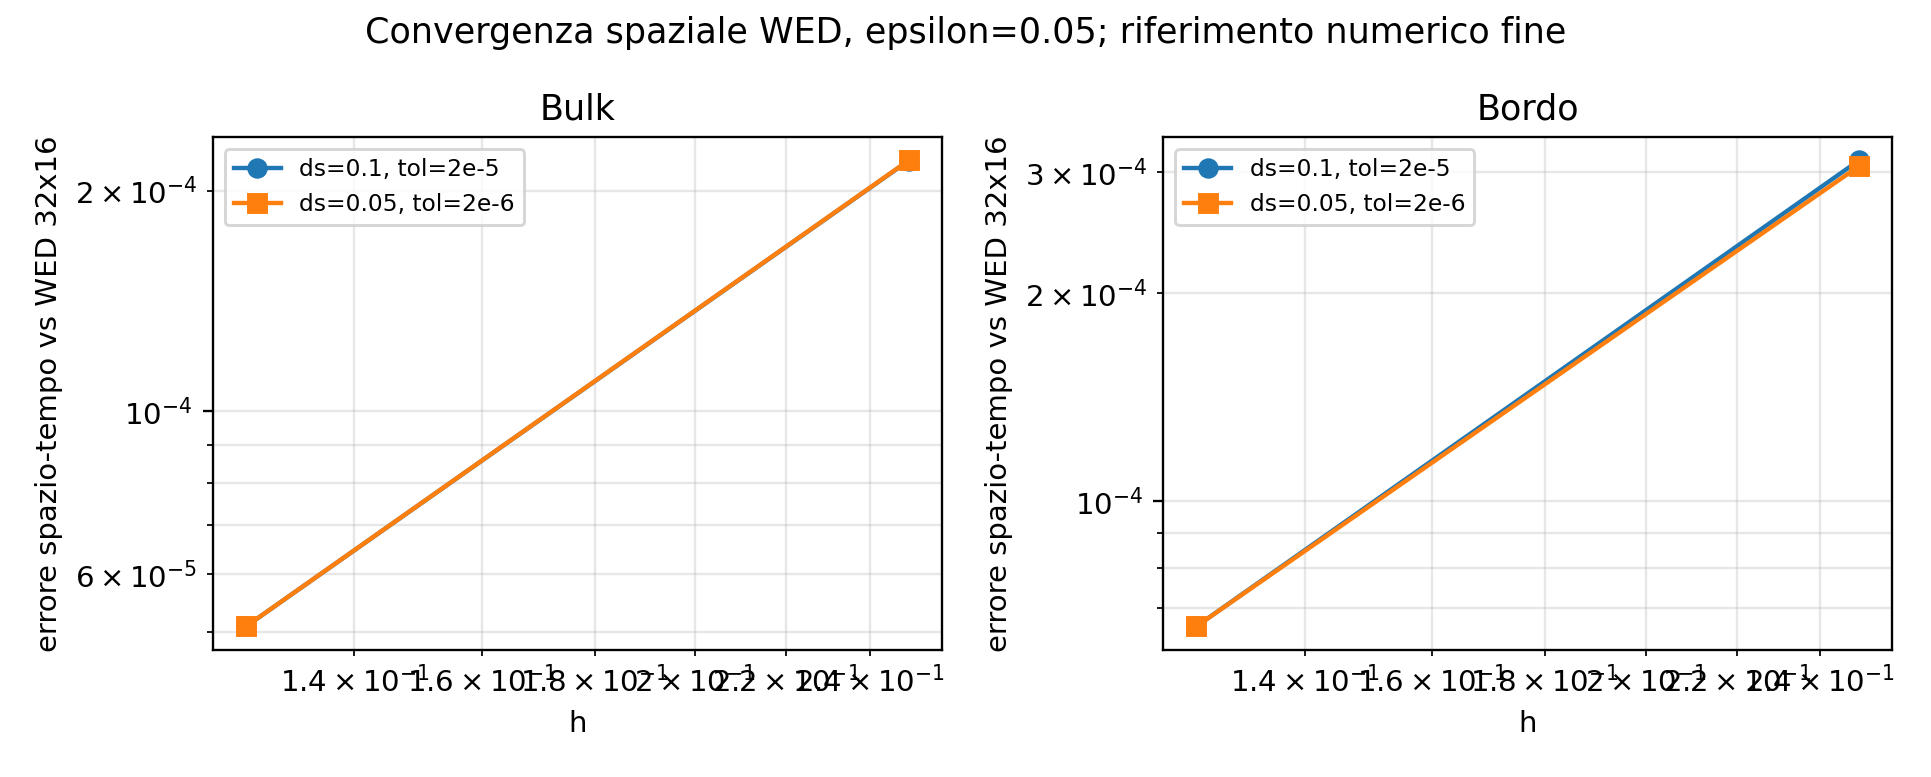
\includegraphics[width=\textwidth]{../stvowu_validation/paper_figures/figure4_mesh.png}
\caption{Bulk and surface errors relative to the $32\times16$ WED path at fixed $\eps$. The fine path is a numerical reference. The two data sets use the $\Delta s$ and tolerances specified in the legend.}
\label{num:fig-mesh}\end{figure}

\subsection{Energy decay}
Figure~\ref{num:fig-energy} reports the direct evolution on $(0,1)^2$, with a $20\times20$ quadrilateral mesh, $u^0(x,y)=0.1+0.05\cos(2\pi x)$, $\beta=1$, $T=0.1$, and $\Delta t=0.00125$. The total energy decreases; no monotonicity is required of its separate bulk and boundary contributions.
\begin{figure}[ht]\centering
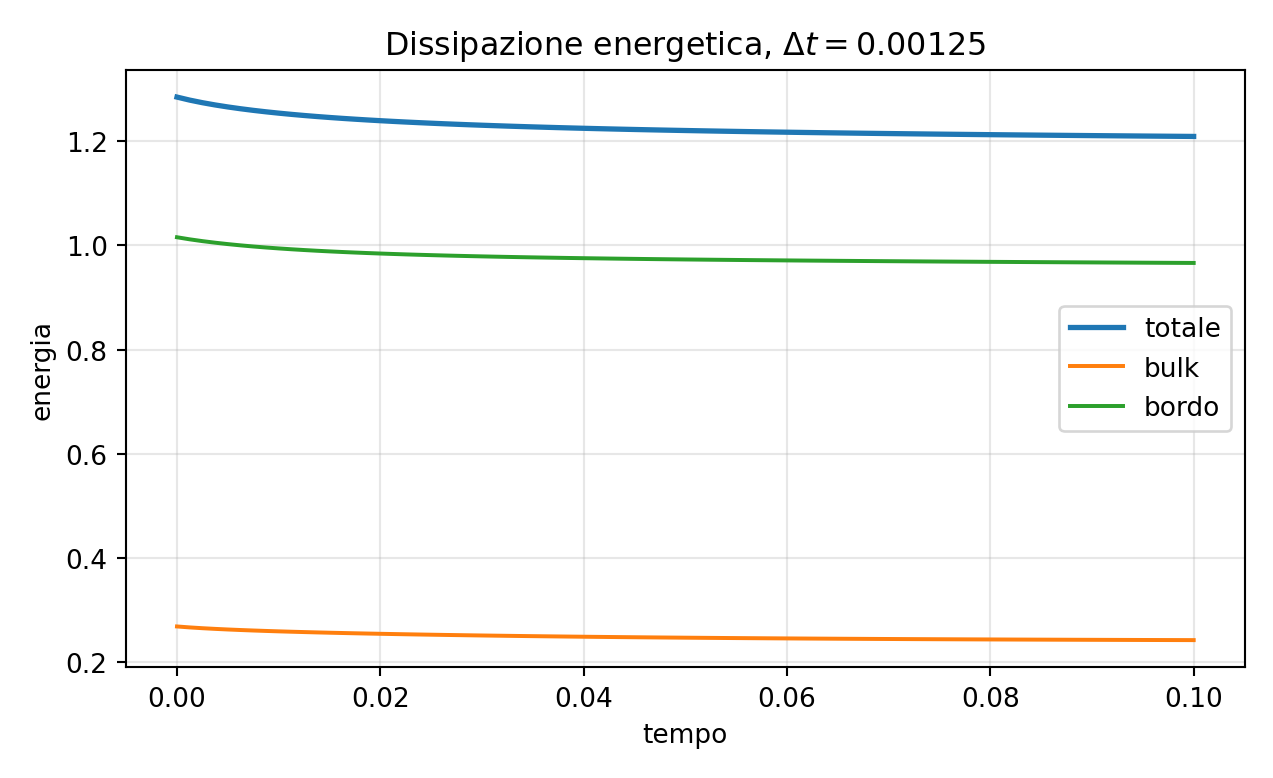
\includegraphics[width=.78\textwidth]{../stvowu_validation/paper_figures/figure5_energy.png}
\caption{Bulk, boundary, and total energy for the direct Allen--Cahn evolution on $(0,1)^2$, mesh $20\times20$, $T=0.1$, and $\Delta t=0.00125$. The total energy decreases, while the individual components need not be monotone.}
\label{num:fig-energy}\end{figure}

\subsection{Dependence on the surface parameter $\beta$}
We vary $\beta\in\{0.5,1,2,5\}$ while keeping the domain $(0,2)\times(0,1)$, mesh $8\times4$, initial profile \eqref{num:initial}, and disabled manufactured source fixed. The direct OOFEM runs use $\Delta t=5\,10^{-4}$ and end at $T=0.02$. The WED runs use $\eps=0.05$, $S_{\max}=4$, $\Delta s=0.1$, tolerance $2\,10^{-5}$, and end at physical time $T=0.2$. Since the final times differ, the two series are presented separately and are not compared pointwise. We denote by $M_\Gamma(T)=|\Gamma|^{-1}\int_\Gamma u^\Gamma(T)\,\d\sigma$ the boundary mean.
\begin{center}\small
\begin{tabular}{rrrrrr}
\hline
Backend, $T$&$\beta$&$M_\Gamma(T)$&$\mathcal E_\Gamma(T)$&$D_\Omega$&$D_\Gamma$\\
\hline
OOFEM, 0.02&0.5&0.202747&0.739877&0.005098&0.018408\\
&1&0.204470&1.423137&0.005238&0.020230\\
&2&0.207956&2.783037&0.006023&0.029831\\
&5&0.218748&6.806088&0.012690&0.109610\\
WED, 0.2&0.5&0.220390&--&--&--\\
&1&0.233905&--&--&--\\
&2&0.264304&--&--&--\\
&5&0.382729&--&--&--\\
\hline
\end{tabular}
\end{center}
The surface energies and dissipations are reported for the direct transient only. The results show sensitivity to $\beta$ for the selected initial condition; no universal monotonicity or relaxation time is asserted.
\begin{figure}[ht]\centering
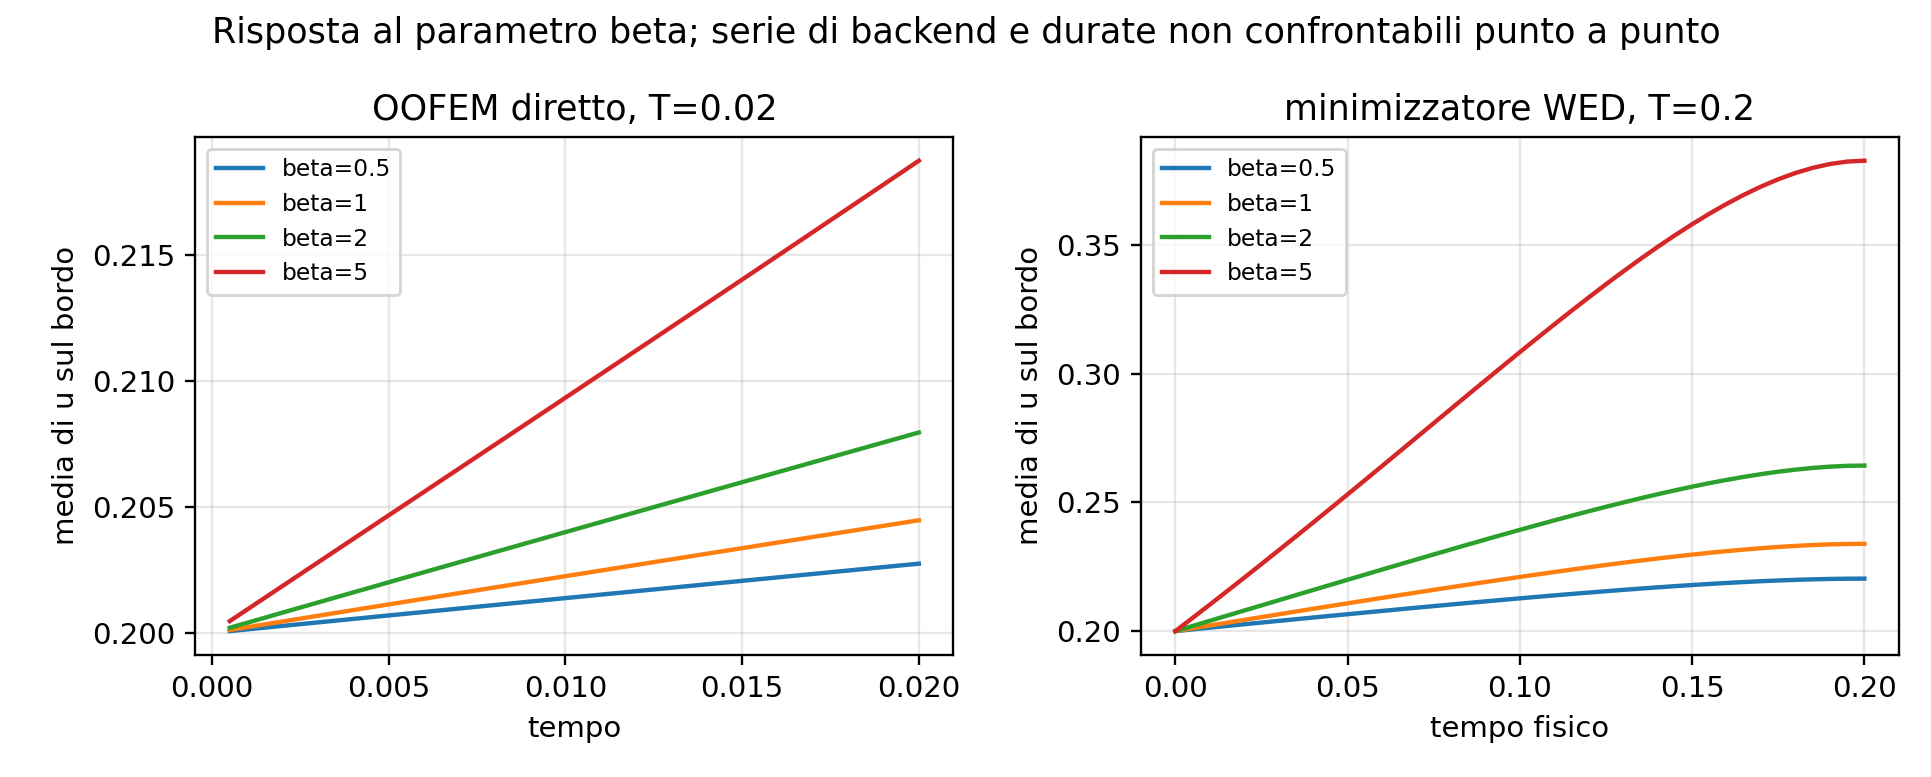
\includegraphics[width=\textwidth]{../stvowu_validation/paper_figures/figure6_beta.png}
\caption{Boundary mean for $\beta=0.5,1,2,5$. Left: direct OOFEM through $T=0.02$, $\Delta t=5\,10^{-4}$. Right: WED minimizer through $T=0.2$, $\eps=0.05$, $S_{\max}=4$, $\Delta s=0.1$. The backends and final times differ.}
\label{num:fig-beta}\end{figure}

\subsection{Scope and reproducibility}
The MMS and energy-balance checks concern the direct solver; the $\eps$, horizon, and mesh studies concern the separate WED Python minimizer. In particular, the MMS test does not validate WED. The comparison with OOFEM at finite $\eps$ includes a regularization bias and is not a pure mesh-convergence test. The reported orders are empirical estimates for the stated benchmarks and do not provide universal convergence results. The computations concern the two-dimensional parabolic model only; the semilinear-wave problem \eqref{allenCahn1} and a triangular $P_1$ benchmark are not included.

Inputs, logs, CSV data, scripts, and figures are archived in the accompanying validation directory. This section source and the six plots are stored there together with the result drivers and parameter tables. The energy residual uses backward differences on saved fields and should be interpreted as a discrete diagnostic. All conclusions are restricted to the reported geometries, initial data, meshes, and tolerances.
 after the
% analytical sections. It uses the article's amsart preamble and equation labels.
\section{Numerical experiments}
\label{section:numerical}

\subsection{Model, discretization, and numerical implementation}
We consider the parabolic Allen--Cahn system \eqref{allenCahn}--\eqref{allenCahnboundary}, with the initial conditions in \eqref{initialConditions}. In the computations, the bulk and surface nonlinearities are chosen as
\begin{equation}
\label{num:potential}
\begin{aligned}
 f(u)&=u^3-u=F'(u), & F(u)&=\frac14(u^2-1)^2,\\
 g(u^\Gamma)&=\beta\bigl((u^\Gamma)^3-u^\Gamma\bigr)=G'(u^\Gamma), &
 G(u^\Gamma)&=\frac{\beta}{4}\bigl((u^\Gamma)^2-1\bigr)^2.
\end{aligned}
\end{equation}
where $\beta>0$ weights the surface potential. The corresponding total energy is
\begin{equation}
\label{num:energy}
\mathcal E(u,u^\Gamma)=\int_\Omega\left(\frac12|\nabla u|^2+F(u)\right)\,\d x
+\int_\Gamma\left(\frac12|\nabla_\Gamma u^\Gamma|^2+G(u^\Gamma)\right)\,\d\sigma.
\end{equation}
All variables and parameters below are dimensionless.

Although the paper treats domains in $\mathbb R^3$, the computations reported here use a two-dimensional rectangular domain $\Omega=(0,2)\times(0,1)$ and its full boundary $\Gamma=\partial\Omega$. The bulk is discretized by bilinear quadrilateral $Q_1$ elements, with the same scalar degrees of freedom used by the boundary line elements. Nine Gauss points are used in each quadrilateral to integrate the cubic reaction term, and three points are used on each line element. The direct evolution problem is solved by the C++ OOFEM transport solver with $\alpha=1$ and input tolerance $\mathrm{rtol}=10^{-11}$. The WED trajectories are computed by a separate Python minimizer; they are not computed by the OOFEM executable. The minimizer uses piecewise-linear time elements, Gaussian quadrature, a free terminal value, and damped sparse Newton iterations. Its stopping tolerance is the infinity norm of the gradient of the rescaled functional, and the maximum number of iterations is 100.

Following the time rescaling used in the proof of the WED result, let $s=t/\eps$. The finite-horizon functional minimized in the computations is
\begin{equation}
\label{num:wed}
\begin{split}
J_{\eps,S_{\max}}(v)=\int_0^{S_{\max}}e^{-s}\bigg[&\frac12\|v_s\|^2_{L^2(\Omega)\oplus L^2(\Gamma)}\\
&+\frac{\eps}{2}\|\nabla v\|^2_{L^2(\Omega)}
+\frac{\eps}{2}\|\nabla_\Gamma v^\Gamma\|^2_{L^2(\Gamma)}\\
&+\eps\int_\Omega F(v)\,\d x
+\eps\int_\Gamma G(v^\Gamma)\,\d\sigma\bigg],\d s,
\end{split}
\end{equation}
subject to $v(0)=u^0$ and $v^\Gamma=v|_\Gamma$. The terminal value at $s=S_{\max}$ is unconstrained. This is a truncated and discretized counterpart of the WED formulation underlying Theorem~\ref{WEDapproach}; the corresponding Euler--Lagrange equation is discussed in \eqref{55b}. The step in physical time satisfies
\begin{equation}
\label{num:dt}
\Delta t=\eps\,\Delta s.
\end{equation}

The nonuniform initial profile used for the WED limit, horizon, spatial, and $\beta$ studies is
\begin{equation}
\label{num:initial}
u^0(x,y)=0.2+0.1\left[\cos\!\left(\frac{\pi x}{2}\right)\cos(\pi y)
+0.25\sin\!\left(\frac{\pi x}{2}\right)\sin(\pi y)\right],
\end{equation}
with $\beta=1$ unless varied explicitly. The manufactured source is switched off for these evolution tests. In the WED limit study, the direct OOFEM trajectory is a numerical comparator, not an exact solution. The MMS test below is the separate comparison with a known exact solution.

\subsection{Verification of the direct solver by a manufactured solution}
We first verify the direct OOFEM solver against the manufactured solution
\begin{equation}
\label{num:mms}
u^*(x,y,t)=0.2+0.1e^{-t}\left[\cos\!\left(\frac{\pi x}{2}\right)\cos(\pi y)
+0.25\sin\!\left(\frac{\pi x}{2}\right)\sin(\pi y)\right],
\end{equation}
with consistent source terms in the bulk and on the boundary. Here $\eps$ is not a parameter of the direct evolution; the time step is $\Delta t=5\,10^{-4}$, the final time is $T=0.02$, and $\beta=1$. The reported nodal RMS error is $e_h=[N^{-1}\sum_{i=1}^N|u_i-u^*(x_i,T)|^2]^{1/2}$. The observed slope $p=\log_2(e_h/e_{h/2})$ is empirical.
\begin{center}\small
\begin{tabular}{rrrrrrr}
\hline
Mesh & Nodes/DoFs & $h$ & Nodal RMS & Maximum error & $\Delta t$ & $p$\\
\hline
$8\times4$ &45&0.250&$7.8821\,10^{-5}$&$1.8014\,10^{-4}$&$5\,10^{-4}$&--\\
$16\times8$&153&0.125&$1.7886\,10^{-5}$&$3.8000\,10^{-5}$&$5\,10^{-4}$&2.140\\
$32\times16$&561&0.0625&$4.3869\,10^{-6}$&$9.4361\,10^{-6}$&$5\,10^{-4}$&2.028\\
\hline
\end{tabular}
\end{center}
The observed order is consistent with second-order spatial convergence for the direct solver in this MMS case. This test verifies the direct solver and does not validate the WED minimizer.

\subsection{Dissipation and the discrete energy balance}
For the unforced gradient-flow system, the formal energy identity associated with \eqref{allenCahn}--\eqref{allenCahnboundary} is
\begin{equation}
\label{num:formal-dissipation}
\frac{\d}{\d t}\mathcal E(u(t),u^\Gamma(t))
=-\|u_t(t)\|_{L^2(\Omega)}^2-\|u_t^\Gamma(t)\|_{L^2(\Gamma)}^2.
\end{equation}
We define the accumulated bulk and boundary dissipations and the balance residual by
\begin{equation}
\label{num:balance}
D_\Omega=\int_0^T\!\int_\Omega|u_t|^2\,\d x\,\d t,\qquad
D_\Gamma=\int_0^T\!\int_\Gamma|u_t^\Gamma|^2\,\d\sigma\,\d t,\qquad
R_E=\mathcal E(T)-\mathcal E(0)+D_\Omega+D_\Gamma.
\end{equation}
The energy-balance runs use $T=0.1$, $\Omega=(0,1)^2$, a $20\times20$ quadrilateral mesh, $u^0(x,y)=0.1+0.05\cos(2\pi x)$, $\beta=1$, and no manufactured source. The values of $u_t$ are approximated by backward differences and the dissipations are evaluated using the FEM mass matrices. Thus, this is a discrete finite-step check, not an analytical proof of stability.
\begin{center}\small
\begin{tabular}{rrrrrrr}
\hline
$\Delta t$&$\mathcal E(0)$&$\mathcal E(T)$&$D_\Omega$&$D_\Gamma$&$R_E$&$|R_E|/\mathcal E(0)$\\
\hline
0.00500&1.284456&1.209120&0.022138&0.047763&$-5.4350\,10^{-3}$&0.004231\\
0.00250&1.284456&1.209018&0.022887&0.049612&$-2.9395\,10^{-3}$&0.002289\\
0.00125&1.284456&1.208967&0.023310&0.050636&$-1.5420\,10^{-3}$&0.001201\\
\hline
\end{tabular}
\end{center}
The residual is negative and its normalized absolute value decreases from $0.423\%$ to $0.120\%$ as the time step is refined. Since $u_t$ and the dissipations are numerically approximated, a nonzero residual at finite step size is expected. Figure~\ref{num:fig-energy} shows the bulk and surface contributions and their sum; no monotonicity is expected of each contribution separately.

\subsection{The limit $\eps\to0$ for WED minimizers}
We compare the WED paths with a direct OOFEM path on the same $8\times4$ mesh. Both are interpolated to the common physical-time window $t\in[0,0.1]$. The bulk and boundary errors are
\begin{equation}
\label{num:errors}
\begin{split}
E_\Omega&=\left(\int_0^{0.1}\|u_{\rm WED}(t)-u_{\rm OOFEM}(t)\|^2_{L^2(\Omega)}\,\d t\right)^{1/2},\\
E_\Gamma&=\left(\int_0^{0.1}\|u^\Gamma_{\rm WED}(t)-u^\Gamma_{\rm OOFEM}(t)\|^2_{L^2(\Gamma)}\,\d t\right)^{1/2}.
\end{split}
\end{equation}
The direct reference uses $\Delta t=10^{-3}$. In the first series, $S_{\max}=12$, $\Delta s=0.1$, tolerance $2\,10^{-5}$, and the mesh are fixed; hence $\Delta t$ varies with $\eps$ by \eqref{num:dt}. In the second series, $\Delta t=0.005$ is fixed and $\Delta s=0.005/\eps$; $S_{\max}=12$, the mesh, and tolerance remain fixed. Every run converges in two Newton iterations. The local slopes are empirical estimates, not theoretical orders.
\begin{center}\scriptsize
\begin{tabular}{llrrrrrrr}
\hline
Series&$\eps$&$\Delta s$&$\Delta t$&$\eps S_{\max}$&$E_\Omega$&$E_\Gamma$&Newton&tol\\
\hline
fixed $\Delta s$&0.1000&0.100&0.0100&1.200&$1.8485\,10^{-3}$&$3.1960\,10^{-3}$&2&$2\,10^{-5}$\\
&0.0500&0.100&0.0050&0.600&$1.1511\,10^{-3}$&$2.0198\,10^{-3}$&2&$2\,10^{-5}$\\
&0.0250&0.100&0.0025&0.300&$6.8730\,10^{-4}$&$1.1978\,10^{-3}$&2&$2\,10^{-5}$\\
&0.0125&0.100&0.00125&0.150&$3.8735\,10^{-4}$&$6.6759\,10^{-4}$&2&$2\,10^{-5}$\\
fixed $\Delta t$&0.1000&0.050&0.0050&1.200&$1.8475\,10^{-3}$&$3.1947\,10^{-3}$&2&$2\,10^{-5}$\\
&0.0500&0.100&0.0050&0.600&$1.1511\,10^{-3}$&$2.0198\,10^{-3}$&2&$2\,10^{-5}$\\
&0.0250&0.200&0.0050&0.300&$6.8614\,10^{-4}$&$1.1959\,10^{-3}$&2&$2\,10^{-5}$\\
&0.0125&0.400&0.0050&0.150&$3.8299\,10^{-4}$&$6.6022\,10^{-4}$&2&$2\,10^{-5}$\\
\hline
\end{tabular}
\end{center}
For fixed $\Delta s$, the bulk/boundary local slopes are $0.68/0.66$, $0.74/0.75$, and $0.83/0.84$. For fixed physical $\Delta t$, they are approximately $0.68/0.66$, $0.75/0.76$, and $0.84/0.86$. The decreasing error trend is similar under both protocols. Keeping $\Delta t$ fixed reduces temporal-step confounding but does not remove all temporal error; for $\eps=0.0125$ it gives the relatively coarse rescaled step $\Delta s=0.4$.

We therefore additionally halve $\Delta s$ from $0.4$ to $0.2$ at $\eps=0.0125$, keeping $S_{\max}=12$, the mesh, and tolerance $2\,10^{-5}$ fixed. Both runs take two Newton iterations. Relative to OOFEM, the bulk error changes from $3.82985\,10^{-4}$ to $3.86483\,10^{-4}$ and the boundary error from $6.60221\,10^{-4}$ to $6.66145\,10^{-4}$, i.e., by about $0.9\%$. The space--time differences between the two WED paths are $4.16\,10^{-6}$ in the bulk and $6.44\,10^{-6}$ on the boundary. The trend is stable to this targeted refinement, while the error against OOFEM does not decrease monotonically under refinement of the time step alone; we do not interpret the slopes as asymptotic orders.
\begin{center}\small
\begin{tabular}{rrrrrr}
\hline
$\Delta s$&$\Delta t$&Newton&$E_\Omega$&$E_\Gamma$&path difference, bulk/boundary\\
\hline
0.4&0.0050&2&$3.82985\,10^{-4}$&$6.60221\,10^{-4}$&reference\\
0.2&0.0025&2&$3.86483\,10^{-4}$&$6.66145\,10^{-4}$&$4.16\,10^{-6}/6.44\,10^{-6}$\\
\hline
\end{tabular}
\end{center}
\begin{figure}[ht]\centering
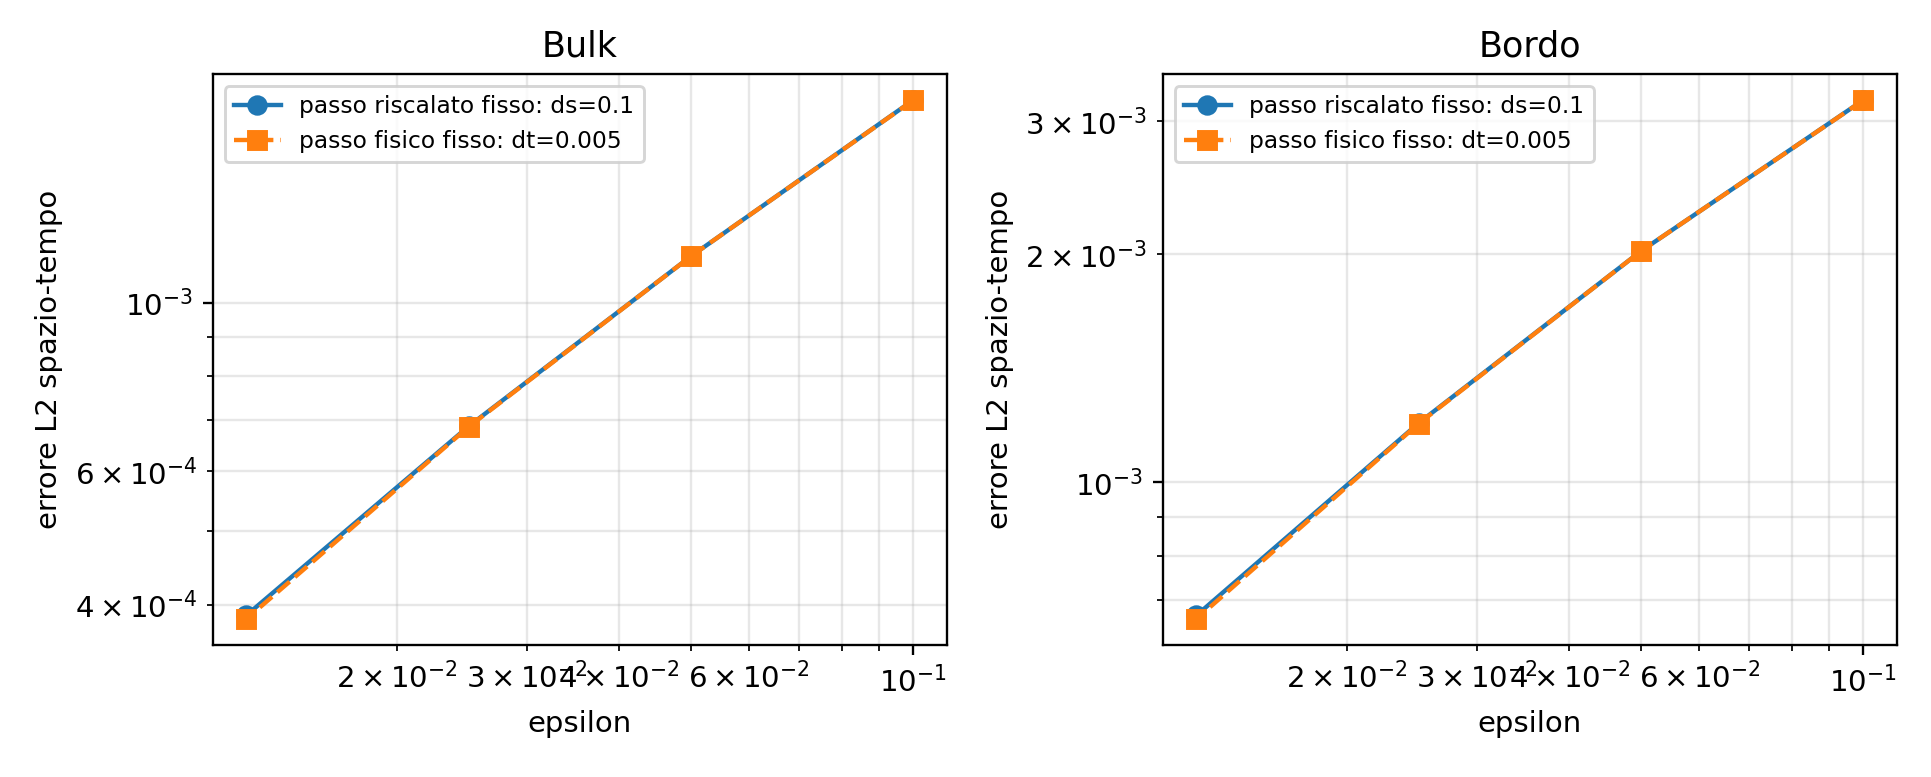
\includegraphics[width=\textwidth]{../stvowu_validation/paper_figures/figure2_epsilon.png}
\caption{Bulk and boundary errors versus $\eps$. Solid lines: fixed $\Delta s=0.1$; dashed lines: fixed physical $\Delta t=0.005$. Errors are integrated over $[0,0.1]$ relative to the direct OOFEM path with $\Delta t=0.001$.}
\label{num:fig-epsilon}\end{figure}

\subsection{Sensitivity to the finite WED horizon}
For $\eps=0.05$, $\Delta s=0.1$, tolerance $2\,10^{-5}$, and the $8\times4$ mesh, we compare $S_{\max}=6,12$ with $18$ over $t\in[0,0.1]$. The reported RMS is the nodal root-mean-square over time,
\[
\mathrm{RMS}_{S_{\max}}=\left[\int_0^{0.1}\frac1N\sum_{i=1}^N|u_i^{S_{\max}}(t)-u_i^{18}(t)|^2\,\d t\right]^{1/2},
\]
and the maximum is the largest nodal difference on the same interval.
\begin{center}\small
\begin{tabular}{rrrr}
\hline
$S_{\max}$&$\Delta t=\eps\Delta s$&RMS vs $S_{\max}=18$&maximum nodal difference\\
\hline
6&0.005&$3.6689\,10^{-5}$&$3.0215\,10^{-4}$\\
12&0.005&$1.5575\,10^{-7}$&$1.1327\,10^{-6}$\\
18&0.005&0 (reference)&0 (reference)\\
\hline
\end{tabular}
\end{center}
This is a truncation-sensitivity check for the stated initial data and time window, not a uniform estimate for other problems.
\begin{figure}[ht]\centering
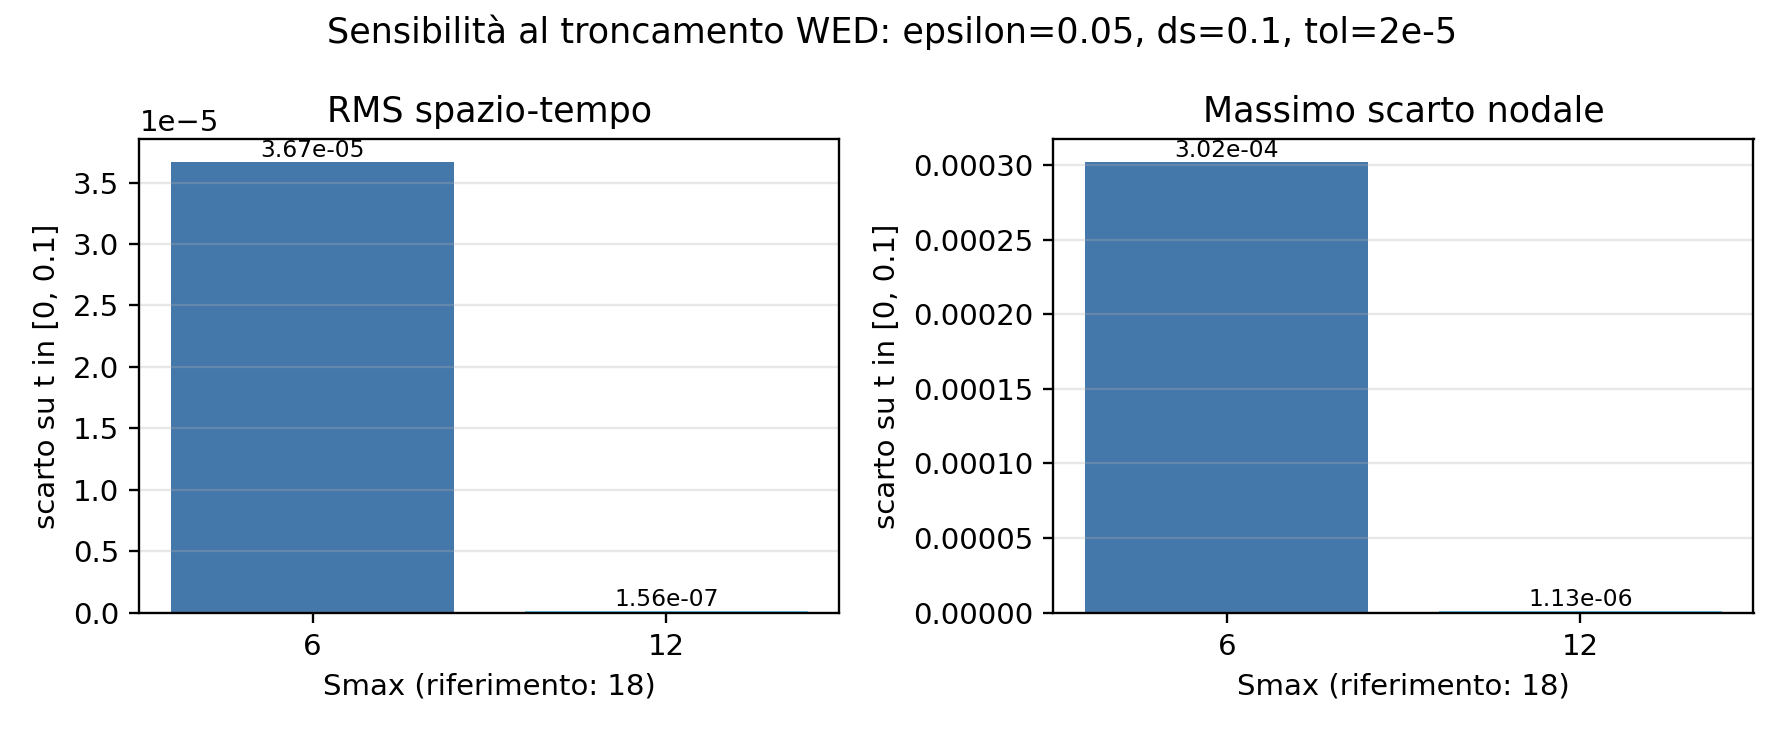
\includegraphics[width=.78\textwidth]{../stvowu_validation/paper_figures/figure3_horizon.png}
\caption{RMS and maximum nodal differences relative to $S_{\max}=18$ for $\eps=0.05$, $\Delta s=0.1$, and $t\in[0,0.1]$.}
\label{num:fig-horizon}\end{figure}

\subsection{Spatial convergence of WED paths}
At fixed $\eps=0.05$, coarse-mesh WED paths are compared against the WED path on the $32\times16$ mesh, used as a numerical reference, not an exact solution. The norms in \eqref{num:errors} are evaluated over $t\in[0,0.1]$. The baseline uses $\Delta s=0.1$ and tolerance $2\,10^{-5}$; the robustness check uses $\Delta s=0.05$ and tolerance $2\,10^{-6}$. The empirical orders are estimated from the two coarse meshes.
\begin{center}\scriptsize
\begin{tabular}{llrrrrr}
\hline
Run&Mesh&$h$&$E_\Omega$&$E_\Gamma$&$p_\Omega$&$p_\Gamma$\\
\hline
baseline&$8\times4$&0.250&$2.1961\,10^{-4}$&$3.1175\,10^{-4}$&2.107&2.243\\
&$16\times8$&0.125&$5.0963\,10^{-5}$&$6.5835\,10^{-5}$&--&--\\
&$32\times16$&0.0625&0 (reference)&0 (reference)&--&--\\
refined&$8\times4$&0.250&$2.1977\,10^{-4}$&$3.0581\,10^{-4}$&2.108&2.216\\
&$16\times8$&0.125&$5.0972\,10^{-5}$&$6.5840\,10^{-5}$&--&--\\
&$32\times16$&0.0625&0 (reference)&0 (reference)&--&--\\
\hline
\end{tabular}
\end{center}
The observed bulk order changes by approximately $0.001$ and the boundary order by $0.028$ under the time-step and tolerance refinement. For these meshes the trend is consistent with second-order spatial convergence and is stable under the tested refinement. WED/OOFEM differences include the finite-$\eps$ bias and are not used to infer spatial order.
\begin{figure}[ht]\centering
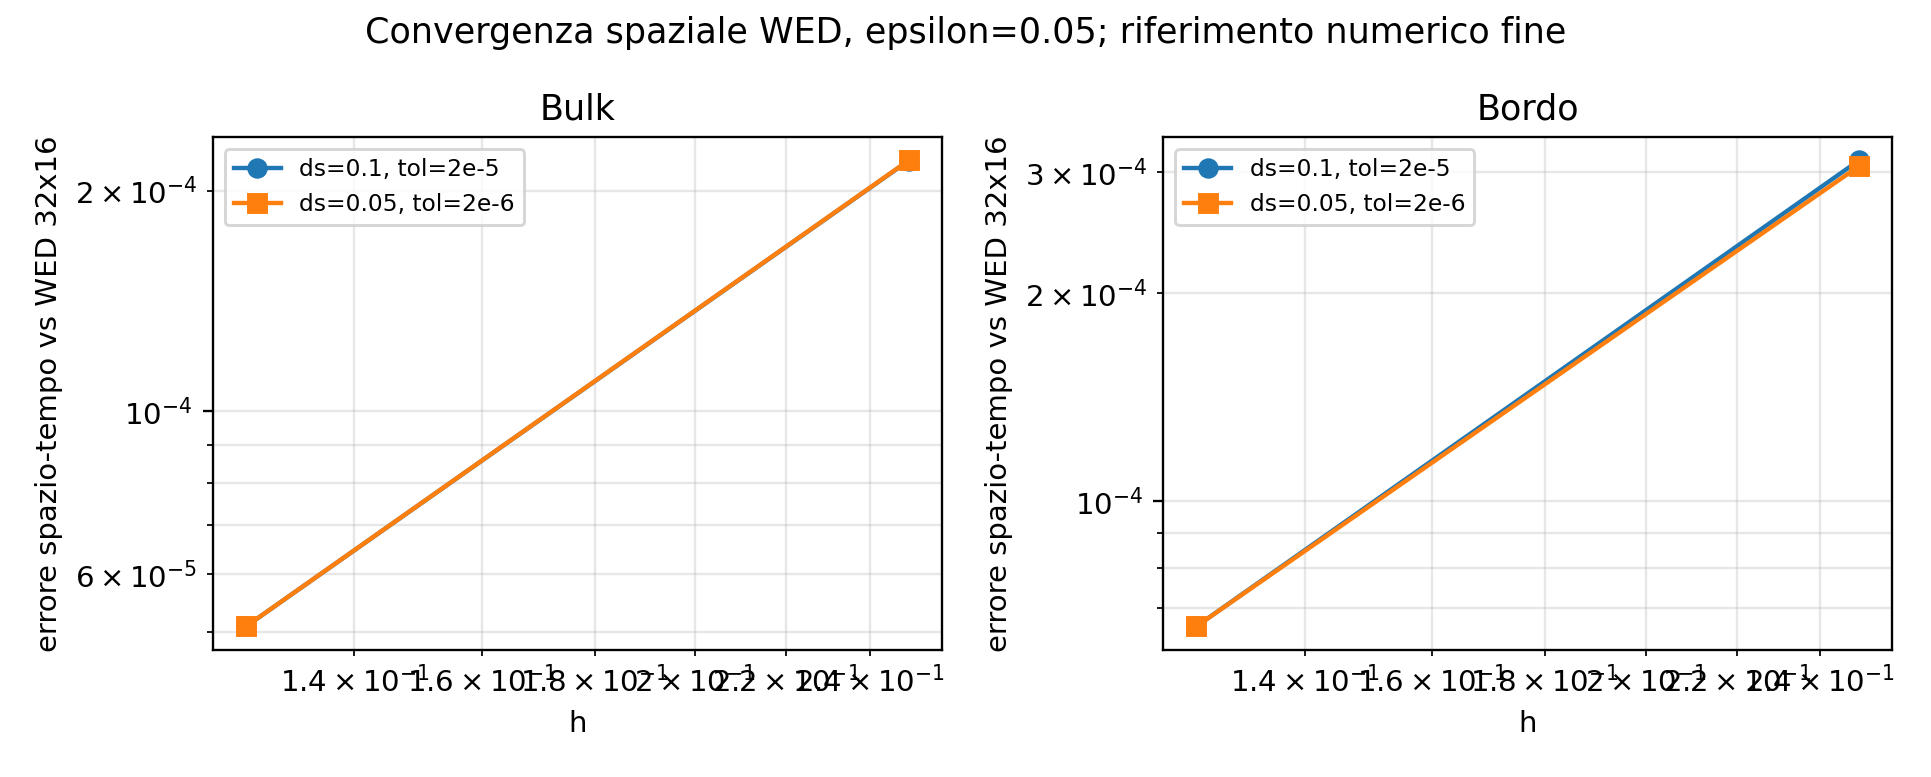
\includegraphics[width=\textwidth]{../stvowu_validation/paper_figures/figure4_mesh.png}
\caption{Bulk and surface errors relative to the $32\times16$ WED path at fixed $\eps$. The fine path is a numerical reference. The two data sets use the $\Delta s$ and tolerances specified in the legend.}
\label{num:fig-mesh}\end{figure}

\subsection{Energy decay}
Figure~\ref{num:fig-energy} reports the direct evolution on $(0,1)^2$, with a $20\times20$ quadrilateral mesh, $u^0(x,y)=0.1+0.05\cos(2\pi x)$, $\beta=1$, $T=0.1$, and $\Delta t=0.00125$. The total energy decreases; no monotonicity is required of its separate bulk and boundary contributions.
\begin{figure}[ht]\centering
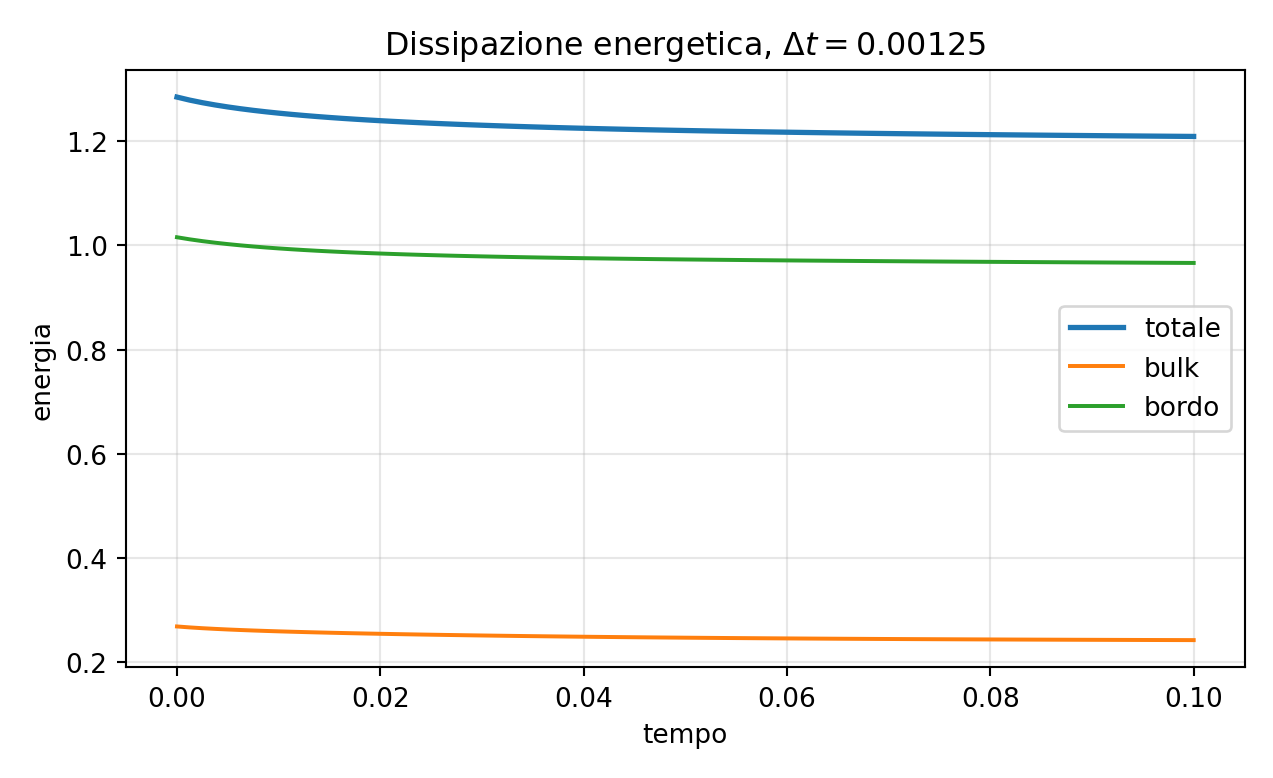
\includegraphics[width=.78\textwidth]{../stvowu_validation/paper_figures/figure5_energy.png}
\caption{Bulk, boundary, and total energy for the direct Allen--Cahn evolution on $(0,1)^2$, mesh $20\times20$, $T=0.1$, and $\Delta t=0.00125$. The total energy decreases, while the individual components need not be monotone.}
\label{num:fig-energy}\end{figure}

\subsection{Dependence on the surface parameter $\beta$}
We vary $\beta\in\{0.5,1,2,5\}$ while keeping the domain $(0,2)\times(0,1)$, mesh $8\times4$, initial profile \eqref{num:initial}, and disabled manufactured source fixed. The direct OOFEM runs use $\Delta t=5\,10^{-4}$ and end at $T=0.02$. The WED runs use $\eps=0.05$, $S_{\max}=4$, $\Delta s=0.1$, tolerance $2\,10^{-5}$, and end at physical time $T=0.2$. Since the final times differ, the two series are presented separately and are not compared pointwise. We denote by $M_\Gamma(T)=|\Gamma|^{-1}\int_\Gamma u^\Gamma(T)\,\d\sigma$ the boundary mean.
\begin{center}\small
\begin{tabular}{rrrrrr}
\hline
Backend, $T$&$\beta$&$M_\Gamma(T)$&$\mathcal E_\Gamma(T)$&$D_\Omega$&$D_\Gamma$\\
\hline
OOFEM, 0.02&0.5&0.202747&0.739877&0.005098&0.018408\\
&1&0.204470&1.423137&0.005238&0.020230\\
&2&0.207956&2.783037&0.006023&0.029831\\
&5&0.218748&6.806088&0.012690&0.109610\\
WED, 0.2&0.5&0.220390&--&--&--\\
&1&0.233905&--&--&--\\
&2&0.264304&--&--&--\\
&5&0.382729&--&--&--\\
\hline
\end{tabular}
\end{center}
The surface energies and dissipations are reported for the direct transient only. The results show sensitivity to $\beta$ for the selected initial condition; no universal monotonicity or relaxation time is asserted.
\begin{figure}[ht]\centering
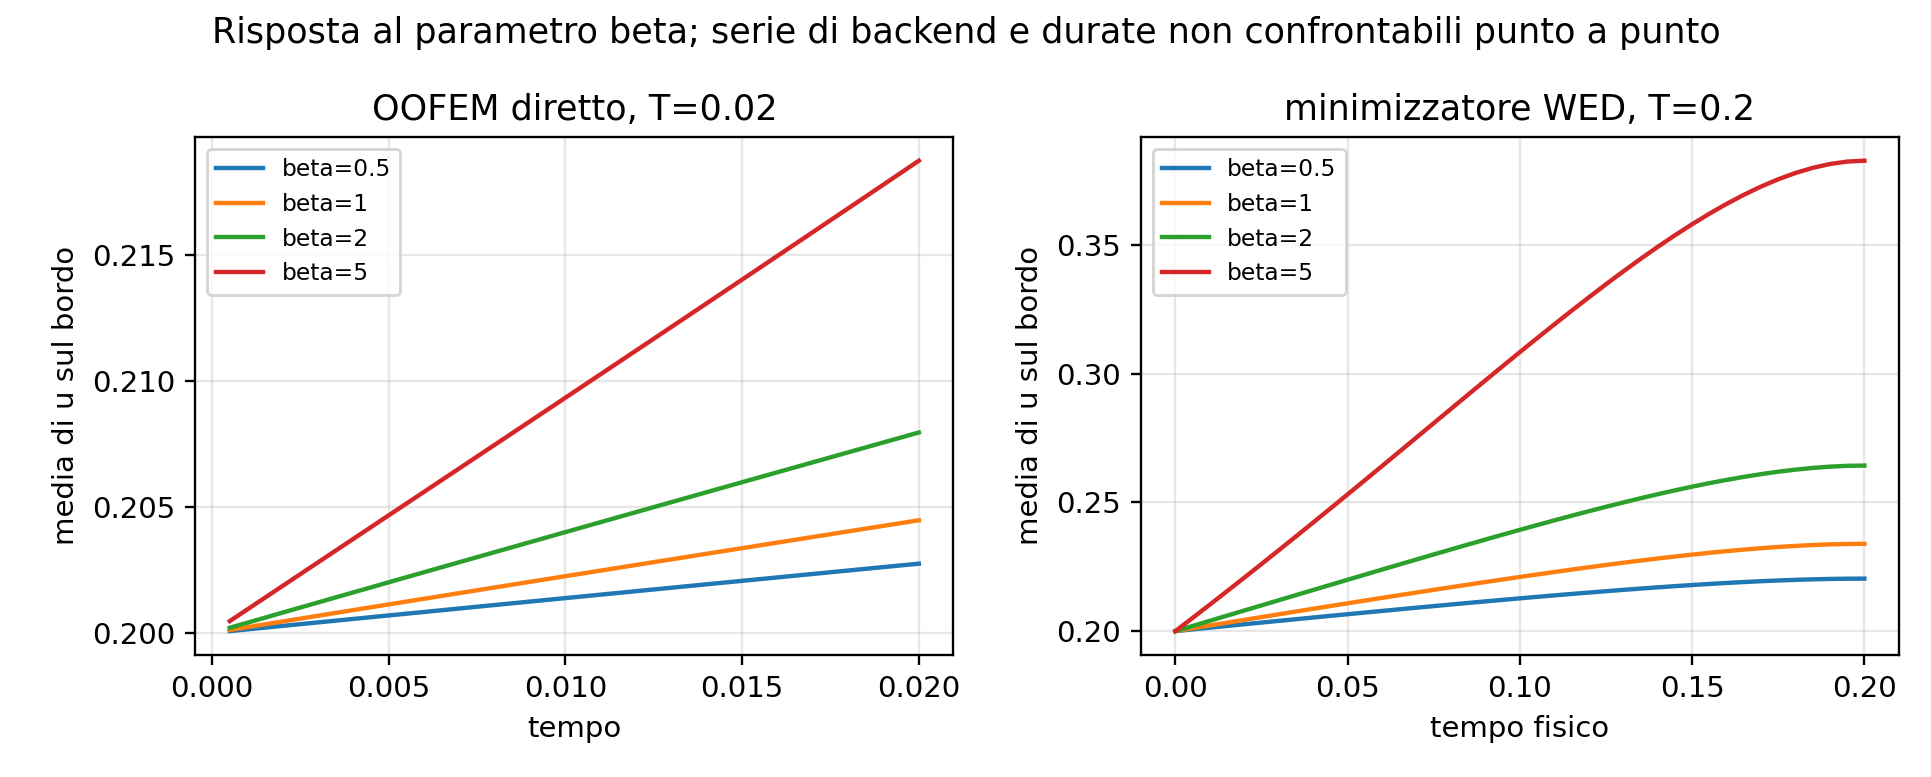
\includegraphics[width=\textwidth]{../stvowu_validation/paper_figures/figure6_beta.png}
\caption{Boundary mean for $\beta=0.5,1,2,5$. Left: direct OOFEM through $T=0.02$, $\Delta t=5\,10^{-4}$. Right: WED minimizer through $T=0.2$, $\eps=0.05$, $S_{\max}=4$, $\Delta s=0.1$. The backends and final times differ.}
\label{num:fig-beta}\end{figure}

\subsection{Scope and reproducibility}
The MMS and energy-balance checks concern the direct solver; the $\eps$, horizon, and mesh studies concern the separate WED Python minimizer. In particular, the MMS test does not validate WED. The comparison with OOFEM at finite $\eps$ includes a regularization bias and is not a pure mesh-convergence test. The reported orders are empirical estimates for the stated benchmarks and do not provide universal convergence results. The computations concern the two-dimensional parabolic model only; the semilinear-wave problem \eqref{allenCahn1} and a triangular $P_1$ benchmark are not included.

Inputs, logs, CSV data, scripts, and figures are archived in the accompanying validation directory. This section source and the six plots are stored there together with the result drivers and parameter tables. The energy residual uses backward differences on saved fields and should be interpreted as a discrete diagnostic. All conclusions are restricted to the reported geometries, initial data, meshes, and tolerances.
 after the
% analytical sections. It uses the article's amsart preamble and equation labels.
\section{Numerical experiments}
\label{section:numerical}

\subsection{Model, discretization, and numerical implementation}
We consider the parabolic Allen--Cahn system \eqref{allenCahn}--\eqref{allenCahnboundary}, with the initial conditions in \eqref{initialConditions}. In the computations, the bulk and surface nonlinearities are chosen as
\begin{equation}
\label{num:potential}
\begin{aligned}
 f(u)&=u^3-u=F'(u), & F(u)&=\frac14(u^2-1)^2,\\
 g(u^\Gamma)&=\beta\bigl((u^\Gamma)^3-u^\Gamma\bigr)=G'(u^\Gamma), &
 G(u^\Gamma)&=\frac{\beta}{4}\bigl((u^\Gamma)^2-1\bigr)^2.
\end{aligned}
\end{equation}
where $\beta>0$ weights the surface potential. The corresponding total energy is
\begin{equation}
\label{num:energy}
\mathcal E(u,u^\Gamma)=\int_\Omega\left(\frac12|\nabla u|^2+F(u)\right)\,\d x
+\int_\Gamma\left(\frac12|\nabla_\Gamma u^\Gamma|^2+G(u^\Gamma)\right)\,\d\sigma.
\end{equation}
All variables and parameters below are dimensionless.

Although the paper treats domains in $\mathbb R^3$, the computations reported here use a two-dimensional rectangular domain $\Omega=(0,2)\times(0,1)$ and its full boundary $\Gamma=\partial\Omega$. The bulk is discretized by bilinear quadrilateral $Q_1$ elements, with the same scalar degrees of freedom used by the boundary line elements. Nine Gauss points are used in each quadrilateral to integrate the cubic reaction term, and three points are used on each line element. The direct evolution problem is solved by the C++ OOFEM transport solver with $\alpha=1$ and input tolerance $\mathrm{rtol}=10^{-11}$. The WED trajectories are computed by a separate Python minimizer; they are not computed by the OOFEM executable. The minimizer uses piecewise-linear time elements, Gaussian quadrature, a free terminal value, and damped sparse Newton iterations. Its stopping tolerance is the infinity norm of the gradient of the rescaled functional, and the maximum number of iterations is 100.

Following the time rescaling used in the proof of the WED result, let $s=t/\eps$. The finite-horizon functional minimized in the computations is
\begin{equation}
\label{num:wed}
\begin{split}
J_{\eps,S_{\max}}(v)=\int_0^{S_{\max}}e^{-s}\bigg[&\frac12\|v_s\|^2_{L^2(\Omega)\oplus L^2(\Gamma)}\\
&+\frac{\eps}{2}\|\nabla v\|^2_{L^2(\Omega)}
+\frac{\eps}{2}\|\nabla_\Gamma v^\Gamma\|^2_{L^2(\Gamma)}\\
&+\eps\int_\Omega F(v)\,\d x
+\eps\int_\Gamma G(v^\Gamma)\,\d\sigma\bigg],\d s,
\end{split}
\end{equation}
subject to $v(0)=u^0$ and $v^\Gamma=v|_\Gamma$. The terminal value at $s=S_{\max}$ is unconstrained. This is a truncated and discretized counterpart of the WED formulation underlying Theorem~\ref{WEDapproach}; the corresponding Euler--Lagrange equation is discussed in \eqref{55b}. The step in physical time satisfies
\begin{equation}
\label{num:dt}
\Delta t=\eps\,\Delta s.
\end{equation}

The nonuniform initial profile used for the WED limit, horizon, spatial, and $\beta$ studies is
\begin{equation}
\label{num:initial}
u^0(x,y)=0.2+0.1\left[\cos\!\left(\frac{\pi x}{2}\right)\cos(\pi y)
+0.25\sin\!\left(\frac{\pi x}{2}\right)\sin(\pi y)\right],
\end{equation}
with $\beta=1$ unless varied explicitly. The manufactured source is switched off for these evolution tests. In the WED limit study, the direct OOFEM trajectory is a numerical comparator, not an exact solution. The MMS test below is the separate comparison with a known exact solution.

\subsection{Verification of the direct solver by a manufactured solution}
We first verify the direct OOFEM solver against the manufactured solution
\begin{equation}
\label{num:mms}
u^*(x,y,t)=0.2+0.1e^{-t}\left[\cos\!\left(\frac{\pi x}{2}\right)\cos(\pi y)
+0.25\sin\!\left(\frac{\pi x}{2}\right)\sin(\pi y)\right],
\end{equation}
with consistent source terms in the bulk and on the boundary. Here $\eps$ is not a parameter of the direct evolution; the time step is $\Delta t=5\,10^{-4}$, the final time is $T=0.02$, and $\beta=1$. The reported nodal RMS error is $e_h=[N^{-1}\sum_{i=1}^N|u_i-u^*(x_i,T)|^2]^{1/2}$. The observed slope $p=\log_2(e_h/e_{h/2})$ is empirical.
\begin{center}\small
\begin{tabular}{rrrrrrr}
\hline
Mesh & Nodes/DoFs & $h$ & Nodal RMS & Maximum error & $\Delta t$ & $p$\\
\hline
$8\times4$ &45&0.250&$7.8821\,10^{-5}$&$1.8014\,10^{-4}$&$5\,10^{-4}$&--\\
$16\times8$&153&0.125&$1.7886\,10^{-5}$&$3.8000\,10^{-5}$&$5\,10^{-4}$&2.140\\
$32\times16$&561&0.0625&$4.3869\,10^{-6}$&$9.4361\,10^{-6}$&$5\,10^{-4}$&2.028\\
\hline
\end{tabular}
\end{center}
The observed order is consistent with second-order spatial convergence for the direct solver in this MMS case. This test verifies the direct solver and does not validate the WED minimizer.

\subsection{Dissipation and the discrete energy balance}
For the unforced gradient-flow system, the formal energy identity associated with \eqref{allenCahn}--\eqref{allenCahnboundary} is
\begin{equation}
\label{num:formal-dissipation}
\frac{\d}{\d t}\mathcal E(u(t),u^\Gamma(t))
=-\|u_t(t)\|_{L^2(\Omega)}^2-\|u_t^\Gamma(t)\|_{L^2(\Gamma)}^2.
\end{equation}
We define the accumulated bulk and boundary dissipations and the balance residual by
\begin{equation}
\label{num:balance}
D_\Omega=\int_0^T\!\int_\Omega|u_t|^2\,\d x\,\d t,\qquad
D_\Gamma=\int_0^T\!\int_\Gamma|u_t^\Gamma|^2\,\d\sigma\,\d t,\qquad
R_E=\mathcal E(T)-\mathcal E(0)+D_\Omega+D_\Gamma.
\end{equation}
The energy-balance runs use $T=0.1$, $\Omega=(0,1)^2$, a $20\times20$ quadrilateral mesh, $u^0(x,y)=0.1+0.05\cos(2\pi x)$, $\beta=1$, and no manufactured source. The values of $u_t$ are approximated by backward differences and the dissipations are evaluated using the FEM mass matrices. Thus, this is a discrete finite-step check, not an analytical proof of stability.
\begin{center}\small
\begin{tabular}{rrrrrrr}
\hline
$\Delta t$&$\mathcal E(0)$&$\mathcal E(T)$&$D_\Omega$&$D_\Gamma$&$R_E$&$|R_E|/\mathcal E(0)$\\
\hline
0.00500&1.284456&1.209120&0.022138&0.047763&$-5.4350\,10^{-3}$&0.004231\\
0.00250&1.284456&1.209018&0.022887&0.049612&$-2.9395\,10^{-3}$&0.002289\\
0.00125&1.284456&1.208967&0.023310&0.050636&$-1.5420\,10^{-3}$&0.001201\\
\hline
\end{tabular}
\end{center}
The residual is negative and its normalized absolute value decreases from $0.423\%$ to $0.120\%$ as the time step is refined. Since $u_t$ and the dissipations are numerically approximated, a nonzero residual at finite step size is expected. Figure~\ref{num:fig-energy} shows the bulk and surface contributions and their sum; no monotonicity is expected of each contribution separately.

\subsection{The limit $\eps\to0$ for WED minimizers}
We compare the WED paths with a direct OOFEM path on the same $8\times4$ mesh. Both are interpolated to the common physical-time window $t\in[0,0.1]$. The bulk and boundary errors are
\begin{equation}
\label{num:errors}
\begin{split}
E_\Omega&=\left(\int_0^{0.1}\|u_{\rm WED}(t)-u_{\rm OOFEM}(t)\|^2_{L^2(\Omega)}\,\d t\right)^{1/2},\\
E_\Gamma&=\left(\int_0^{0.1}\|u^\Gamma_{\rm WED}(t)-u^\Gamma_{\rm OOFEM}(t)\|^2_{L^2(\Gamma)}\,\d t\right)^{1/2}.
\end{split}
\end{equation}
The direct reference uses $\Delta t=10^{-3}$. In the first series, $S_{\max}=12$, $\Delta s=0.1$, tolerance $2\,10^{-5}$, and the mesh are fixed; hence $\Delta t$ varies with $\eps$ by \eqref{num:dt}. In the second series, $\Delta t=0.005$ is fixed and $\Delta s=0.005/\eps$; $S_{\max}=12$, the mesh, and tolerance remain fixed. Every run converges in two Newton iterations. The local slopes are empirical estimates, not theoretical orders.
\begin{center}\scriptsize
\begin{tabular}{llrrrrrrr}
\hline
Series&$\eps$&$\Delta s$&$\Delta t$&$\eps S_{\max}$&$E_\Omega$&$E_\Gamma$&Newton&tol\\
\hline
fixed $\Delta s$&0.1000&0.100&0.0100&1.200&$1.8485\,10^{-3}$&$3.1960\,10^{-3}$&2&$2\,10^{-5}$\\
&0.0500&0.100&0.0050&0.600&$1.1511\,10^{-3}$&$2.0198\,10^{-3}$&2&$2\,10^{-5}$\\
&0.0250&0.100&0.0025&0.300&$6.8730\,10^{-4}$&$1.1978\,10^{-3}$&2&$2\,10^{-5}$\\
&0.0125&0.100&0.00125&0.150&$3.8735\,10^{-4}$&$6.6759\,10^{-4}$&2&$2\,10^{-5}$\\
fixed $\Delta t$&0.1000&0.050&0.0050&1.200&$1.8475\,10^{-3}$&$3.1947\,10^{-3}$&2&$2\,10^{-5}$\\
&0.0500&0.100&0.0050&0.600&$1.1511\,10^{-3}$&$2.0198\,10^{-3}$&2&$2\,10^{-5}$\\
&0.0250&0.200&0.0050&0.300&$6.8614\,10^{-4}$&$1.1959\,10^{-3}$&2&$2\,10^{-5}$\\
&0.0125&0.400&0.0050&0.150&$3.8299\,10^{-4}$&$6.6022\,10^{-4}$&2&$2\,10^{-5}$\\
\hline
\end{tabular}
\end{center}
For fixed $\Delta s$, the bulk/boundary local slopes are $0.68/0.66$, $0.74/0.75$, and $0.83/0.84$. For fixed physical $\Delta t$, they are approximately $0.68/0.66$, $0.75/0.76$, and $0.84/0.86$. The decreasing error trend is similar under both protocols. Keeping $\Delta t$ fixed reduces temporal-step confounding but does not remove all temporal error; for $\eps=0.0125$ it gives the relatively coarse rescaled step $\Delta s=0.4$.

We therefore additionally halve $\Delta s$ from $0.4$ to $0.2$ at $\eps=0.0125$, keeping $S_{\max}=12$, the mesh, and tolerance $2\,10^{-5}$ fixed. Both runs take two Newton iterations. Relative to OOFEM, the bulk error changes from $3.82985\,10^{-4}$ to $3.86483\,10^{-4}$ and the boundary error from $6.60221\,10^{-4}$ to $6.66145\,10^{-4}$, i.e., by about $0.9\%$. The space--time differences between the two WED paths are $4.16\,10^{-6}$ in the bulk and $6.44\,10^{-6}$ on the boundary. The trend is stable to this targeted refinement, while the error against OOFEM does not decrease monotonically under refinement of the time step alone; we do not interpret the slopes as asymptotic orders.
\begin{center}\small
\begin{tabular}{rrrrrr}
\hline
$\Delta s$&$\Delta t$&Newton&$E_\Omega$&$E_\Gamma$&path difference, bulk/boundary\\
\hline
0.4&0.0050&2&$3.82985\,10^{-4}$&$6.60221\,10^{-4}$&reference\\
0.2&0.0025&2&$3.86483\,10^{-4}$&$6.66145\,10^{-4}$&$4.16\,10^{-6}/6.44\,10^{-6}$\\
\hline
\end{tabular}
\end{center}
\begin{figure}[ht]\centering
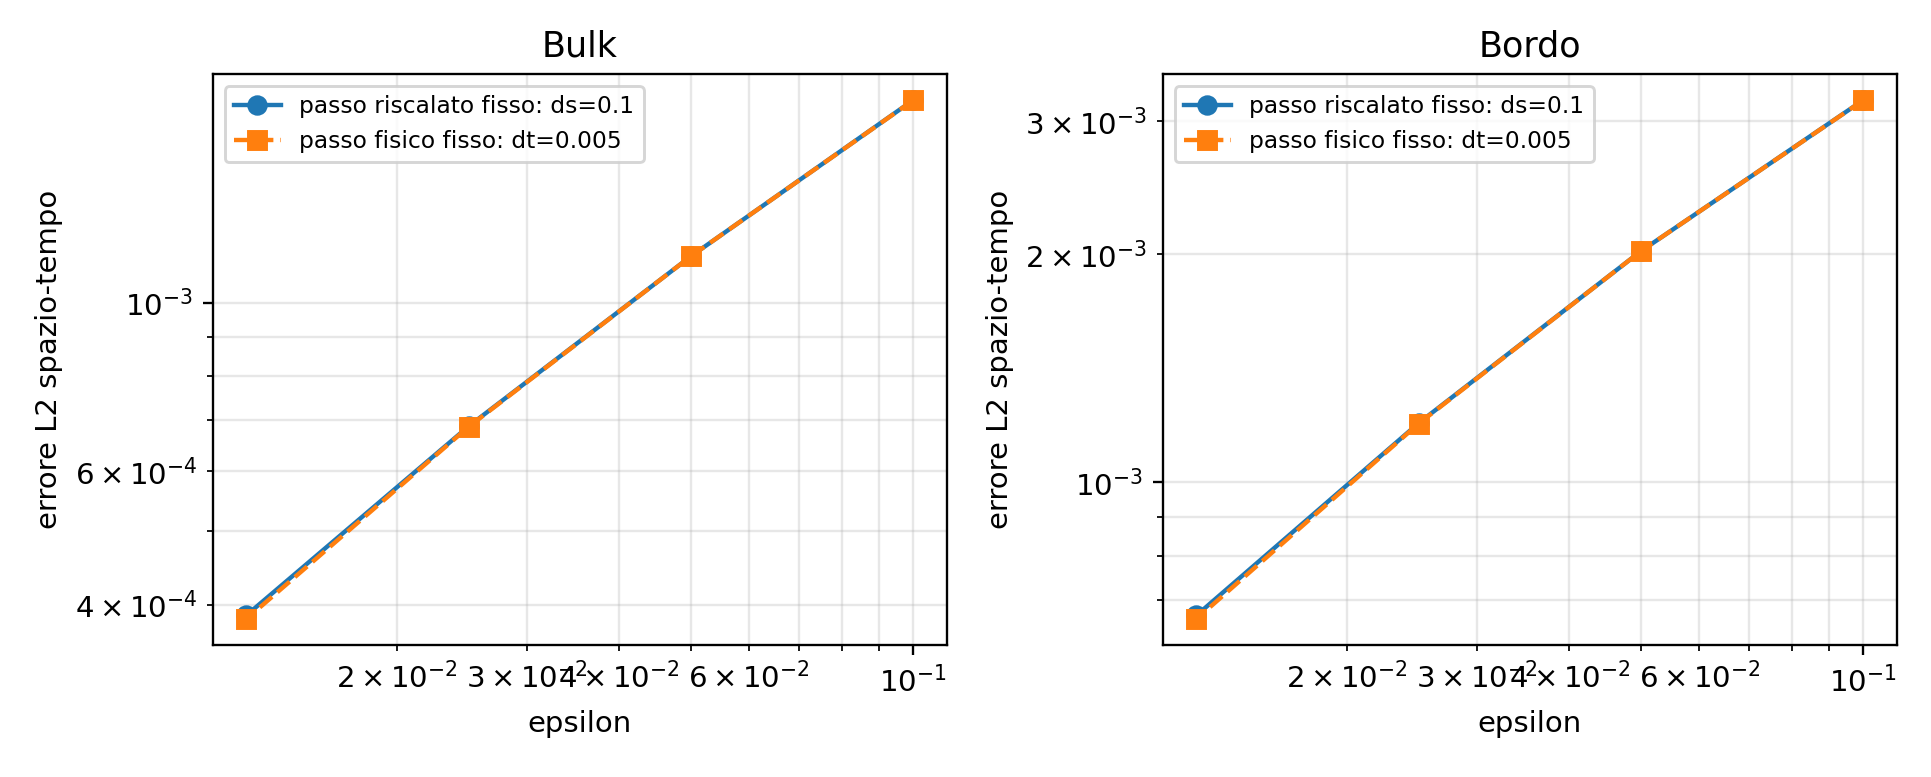
\includegraphics[width=\textwidth]{../stvowu_validation/paper_figures/figure2_epsilon.png}
\caption{Bulk and boundary errors versus $\eps$. Solid lines: fixed $\Delta s=0.1$; dashed lines: fixed physical $\Delta t=0.005$. Errors are integrated over $[0,0.1]$ relative to the direct OOFEM path with $\Delta t=0.001$.}
\label{num:fig-epsilon}\end{figure}

\subsection{Sensitivity to the finite WED horizon}
For $\eps=0.05$, $\Delta s=0.1$, tolerance $2\,10^{-5}$, and the $8\times4$ mesh, we compare $S_{\max}=6,12$ with $18$ over $t\in[0,0.1]$. The reported RMS is the nodal root-mean-square over time,
\[
\mathrm{RMS}_{S_{\max}}=\left[\int_0^{0.1}\frac1N\sum_{i=1}^N|u_i^{S_{\max}}(t)-u_i^{18}(t)|^2\,\d t\right]^{1/2},
\]
and the maximum is the largest nodal difference on the same interval.
\begin{center}\small
\begin{tabular}{rrrr}
\hline
$S_{\max}$&$\Delta t=\eps\Delta s$&RMS vs $S_{\max}=18$&maximum nodal difference\\
\hline
6&0.005&$3.6689\,10^{-5}$&$3.0215\,10^{-4}$\\
12&0.005&$1.5575\,10^{-7}$&$1.1327\,10^{-6}$\\
18&0.005&0 (reference)&0 (reference)\\
\hline
\end{tabular}
\end{center}
This is a truncation-sensitivity check for the stated initial data and time window, not a uniform estimate for other problems.
\begin{figure}[ht]\centering
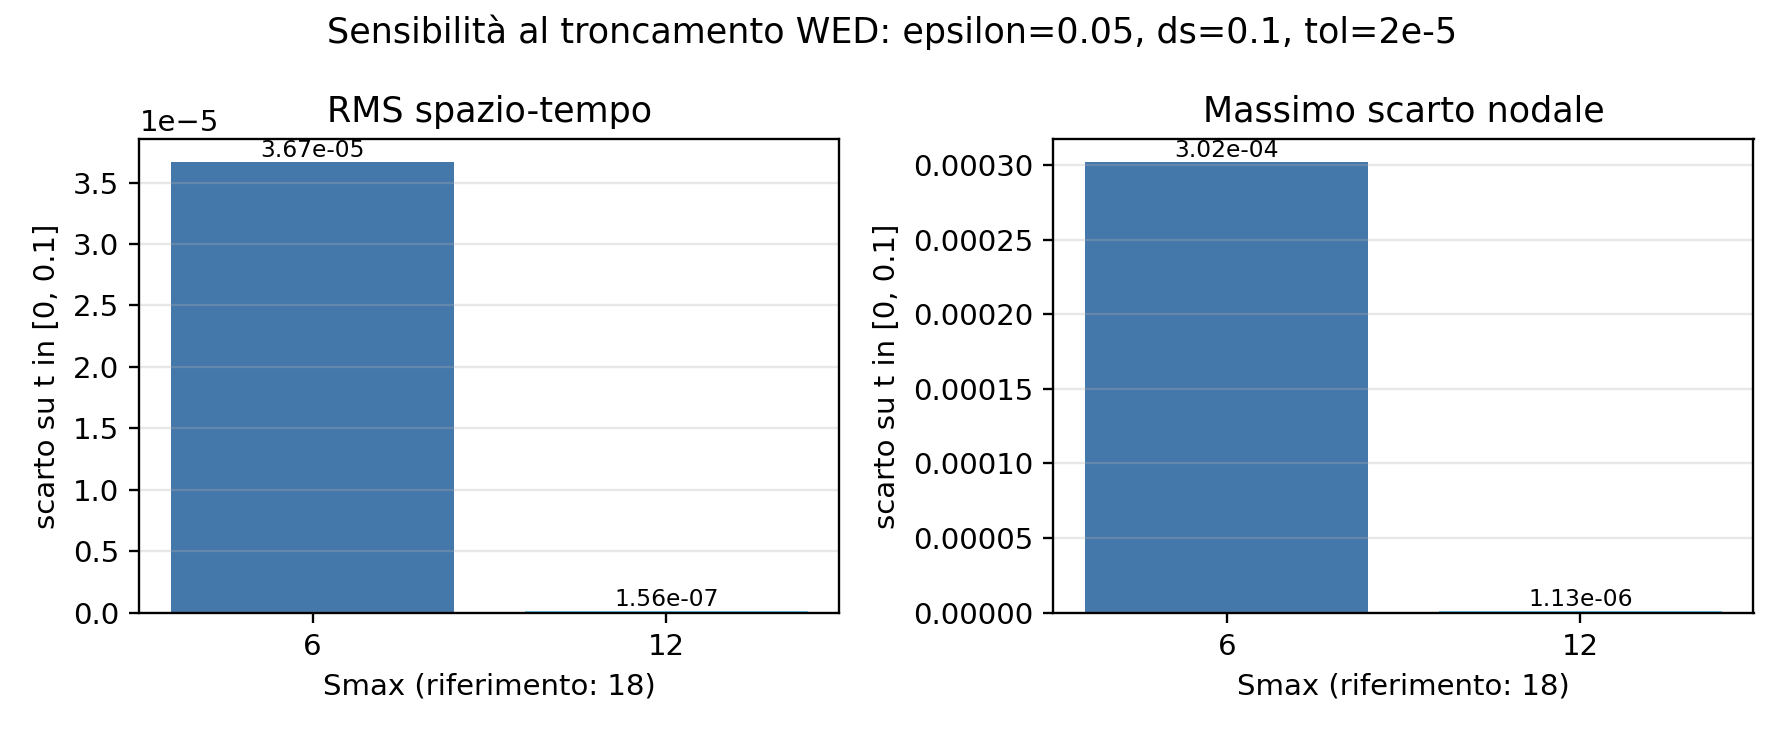
\includegraphics[width=.78\textwidth]{../stvowu_validation/paper_figures/figure3_horizon.png}
\caption{RMS and maximum nodal differences relative to $S_{\max}=18$ for $\eps=0.05$, $\Delta s=0.1$, and $t\in[0,0.1]$.}
\label{num:fig-horizon}\end{figure}

\subsection{Spatial convergence of WED paths}
At fixed $\eps=0.05$, coarse-mesh WED paths are compared against the WED path on the $32\times16$ mesh, used as a numerical reference, not an exact solution. The norms in \eqref{num:errors} are evaluated over $t\in[0,0.1]$. The baseline uses $\Delta s=0.1$ and tolerance $2\,10^{-5}$; the robustness check uses $\Delta s=0.05$ and tolerance $2\,10^{-6}$. The empirical orders are estimated from the two coarse meshes.
\begin{center}\scriptsize
\begin{tabular}{llrrrrr}
\hline
Run&Mesh&$h$&$E_\Omega$&$E_\Gamma$&$p_\Omega$&$p_\Gamma$\\
\hline
baseline&$8\times4$&0.250&$2.1961\,10^{-4}$&$3.1175\,10^{-4}$&2.107&2.243\\
&$16\times8$&0.125&$5.0963\,10^{-5}$&$6.5835\,10^{-5}$&--&--\\
&$32\times16$&0.0625&0 (reference)&0 (reference)&--&--\\
refined&$8\times4$&0.250&$2.1977\,10^{-4}$&$3.0581\,10^{-4}$&2.108&2.216\\
&$16\times8$&0.125&$5.0972\,10^{-5}$&$6.5840\,10^{-5}$&--&--\\
&$32\times16$&0.0625&0 (reference)&0 (reference)&--&--\\
\hline
\end{tabular}
\end{center}
The observed bulk order changes by approximately $0.001$ and the boundary order by $0.028$ under the time-step and tolerance refinement. For these meshes the trend is consistent with second-order spatial convergence and is stable under the tested refinement. WED/OOFEM differences include the finite-$\eps$ bias and are not used to infer spatial order.
\begin{figure}[ht]\centering
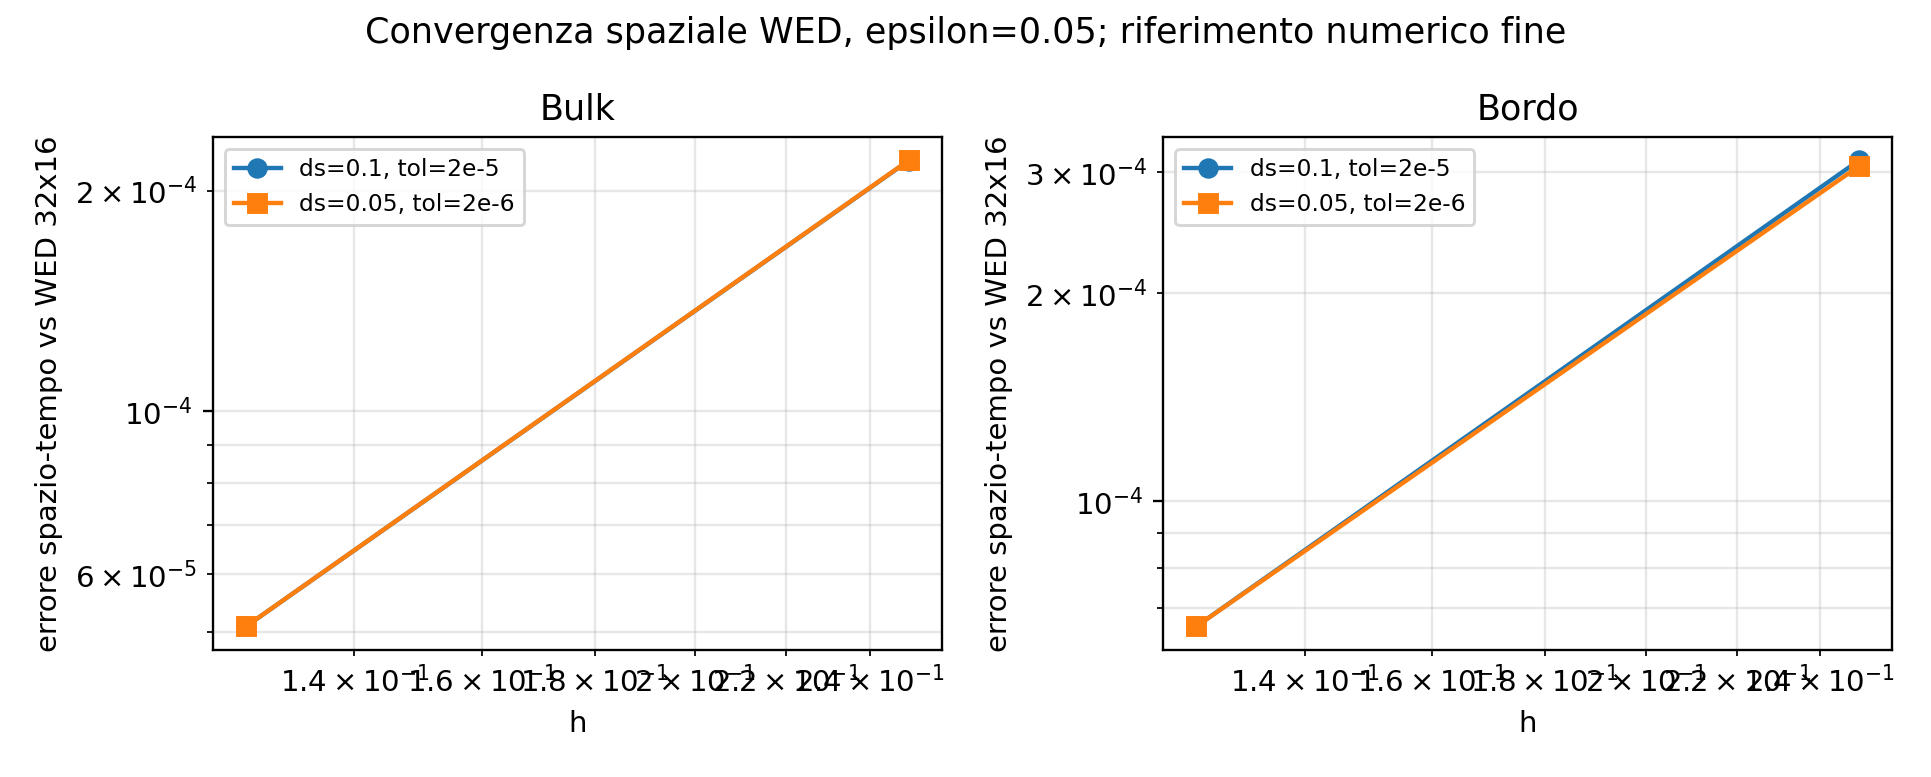
\includegraphics[width=\textwidth]{../stvowu_validation/paper_figures/figure4_mesh.png}
\caption{Bulk and surface errors relative to the $32\times16$ WED path at fixed $\eps$. The fine path is a numerical reference. The two data sets use the $\Delta s$ and tolerances specified in the legend.}
\label{num:fig-mesh}\end{figure}

\subsection{Energy decay}
Figure~\ref{num:fig-energy} reports the direct evolution on $(0,1)^2$, with a $20\times20$ quadrilateral mesh, $u^0(x,y)=0.1+0.05\cos(2\pi x)$, $\beta=1$, $T=0.1$, and $\Delta t=0.00125$. The total energy decreases; no monotonicity is required of its separate bulk and boundary contributions.
\begin{figure}[ht]\centering
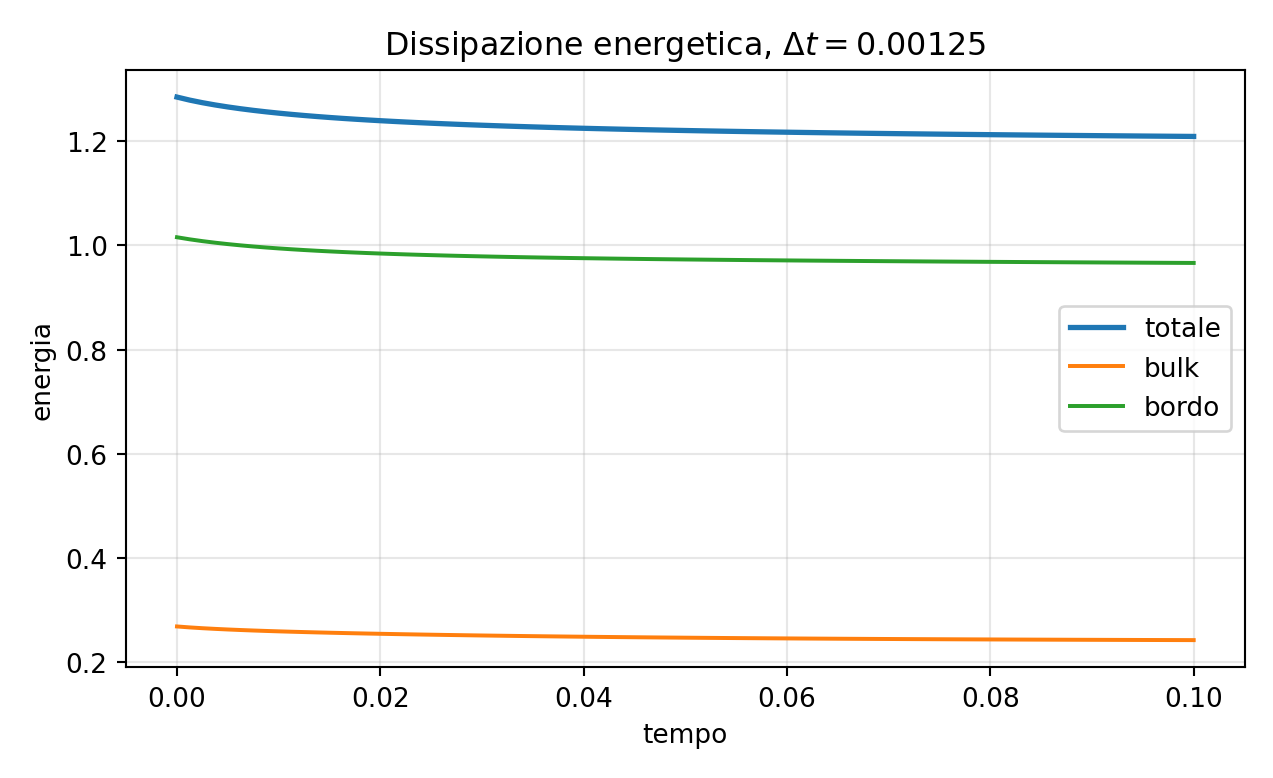
\includegraphics[width=.78\textwidth]{../stvowu_validation/paper_figures/figure5_energy.png}
\caption{Bulk, boundary, and total energy for the direct Allen--Cahn evolution on $(0,1)^2$, mesh $20\times20$, $T=0.1$, and $\Delta t=0.00125$. The total energy decreases, while the individual components need not be monotone.}
\label{num:fig-energy}\end{figure}

\subsection{Dependence on the surface parameter $\beta$}
We vary $\beta\in\{0.5,1,2,5\}$ while keeping the domain $(0,2)\times(0,1)$, mesh $8\times4$, initial profile \eqref{num:initial}, and disabled manufactured source fixed. The direct OOFEM runs use $\Delta t=5\,10^{-4}$ and end at $T=0.02$. The WED runs use $\eps=0.05$, $S_{\max}=4$, $\Delta s=0.1$, tolerance $2\,10^{-5}$, and end at physical time $T=0.2$. Since the final times differ, the two series are presented separately and are not compared pointwise. We denote by $M_\Gamma(T)=|\Gamma|^{-1}\int_\Gamma u^\Gamma(T)\,\d\sigma$ the boundary mean.
\begin{center}\small
\begin{tabular}{rrrrrr}
\hline
Backend, $T$&$\beta$&$M_\Gamma(T)$&$\mathcal E_\Gamma(T)$&$D_\Omega$&$D_\Gamma$\\
\hline
OOFEM, 0.02&0.5&0.202747&0.739877&0.005098&0.018408\\
&1&0.204470&1.423137&0.005238&0.020230\\
&2&0.207956&2.783037&0.006023&0.029831\\
&5&0.218748&6.806088&0.012690&0.109610\\
WED, 0.2&0.5&0.220390&--&--&--\\
&1&0.233905&--&--&--\\
&2&0.264304&--&--&--\\
&5&0.382729&--&--&--\\
\hline
\end{tabular}
\end{center}
The surface energies and dissipations are reported for the direct transient only. The results show sensitivity to $\beta$ for the selected initial condition; no universal monotonicity or relaxation time is asserted.
\begin{figure}[ht]\centering
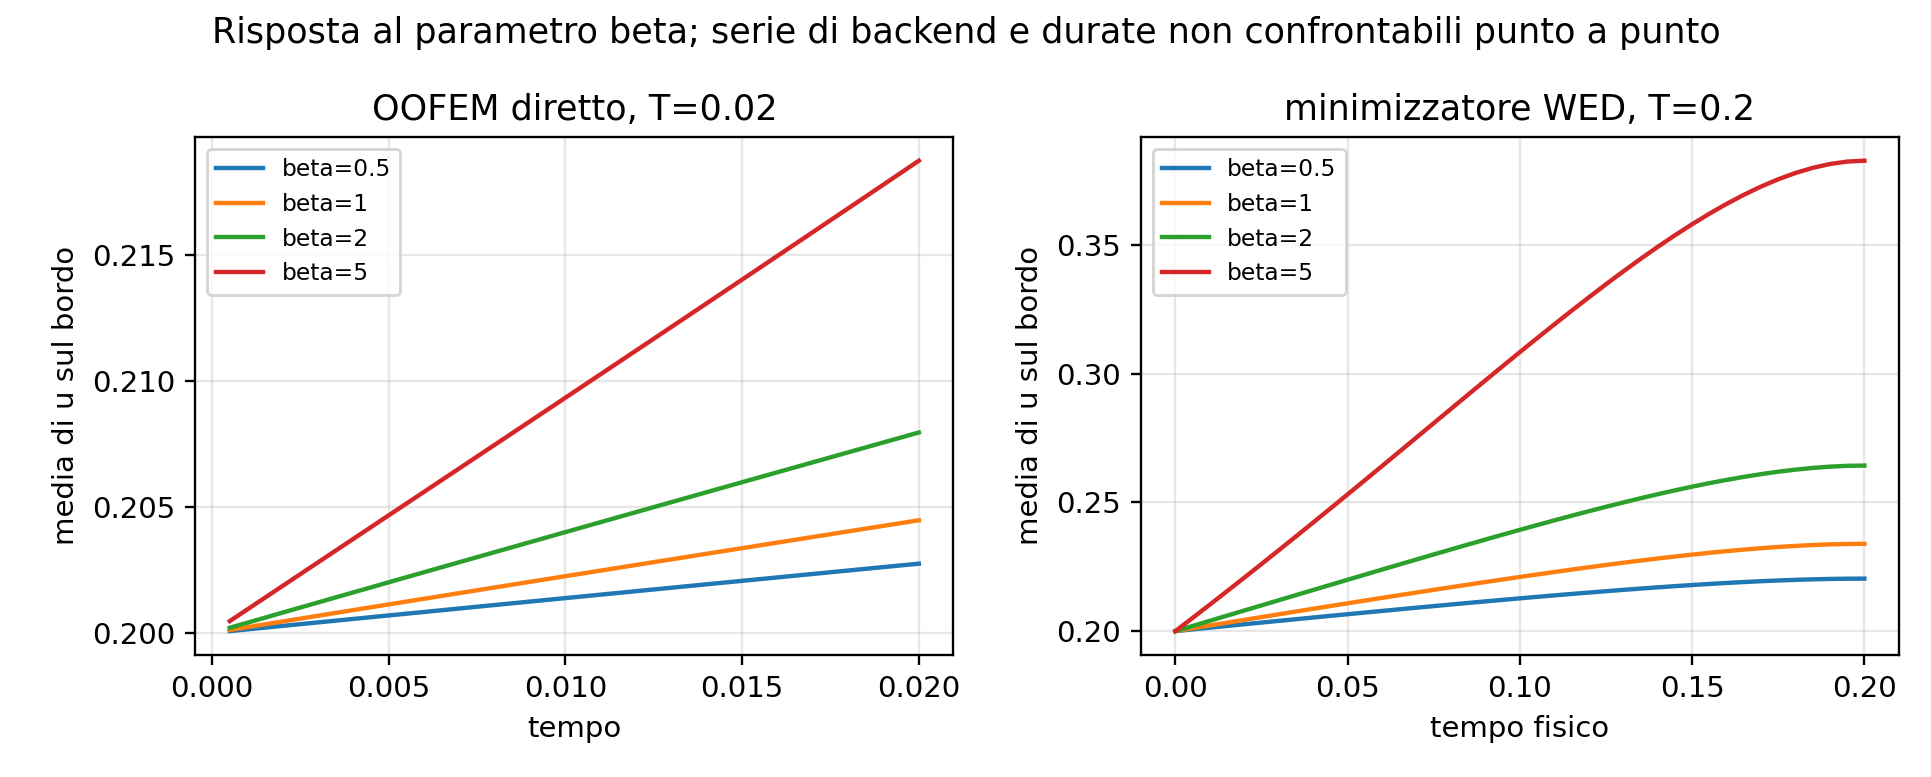
\includegraphics[width=\textwidth]{../stvowu_validation/paper_figures/figure6_beta.png}
\caption{Boundary mean for $\beta=0.5,1,2,5$. Left: direct OOFEM through $T=0.02$, $\Delta t=5\,10^{-4}$. Right: WED minimizer through $T=0.2$, $\eps=0.05$, $S_{\max}=4$, $\Delta s=0.1$. The backends and final times differ.}
\label{num:fig-beta}\end{figure}

\subsection{Scope and reproducibility}
The MMS and energy-balance checks concern the direct solver; the $\eps$, horizon, and mesh studies concern the separate WED Python minimizer. In particular, the MMS test does not validate WED. The comparison with OOFEM at finite $\eps$ includes a regularization bias and is not a pure mesh-convergence test. The reported orders are empirical estimates for the stated benchmarks and do not provide universal convergence results. The computations concern the two-dimensional parabolic model only; the semilinear-wave problem \eqref{allenCahn1} and a triangular $P_1$ benchmark are not included.

Inputs, logs, CSV data, scripts, and figures are archived in the accompanying validation directory. This section source and the six plots are stored there together with the result drivers and parameter tables. The energy residual uses backward differences on saved fields and should be interpreted as a discrete diagnostic. All conclusions are restricted to the reported geometries, initial data, meshes, and tolerances.
